\newif\ifpaper
\paperfalse
% TEMPLATE for Usenix papers, specifically to meet requirements of
%  USENIX '05
% originally a template for producing IEEE-format articles using LaTeX.
%   written by Matthew Ward, CS Department, Worcester Polytechnic Institute.
% adapted by David Beazley for his excellent SWIG paper in Proceedings,
%   Tcl 96
% turned into a smartass generic template by De Clarke, with thanks to
%   both the above pioneers
% use at your own risk.  Complaints to /dev/null.
% make it two column with no page numbering, default is 10 point

% Munged by Fred Douglis <douglis@research.att.com> 10/97 to separate
% the .sty file from the LaTeX source template, so that people can
% more easily include the .sty file into an existing document.  Also
% changed to more closely follow the style guidelines as represented
% by the Word sample file. 

% Note that since 2010, USENIX does not require endnotes. If you want
% foot of page notes, don't include the endnotes package in the 
% usepackage command, below.

% This version uses the latex2e styles, not the very ancient 2.09 stuff.
\documentclass[letterpaper,twocolumn,10pt]{article}
\usepackage{usenix2019,epsfig,endnotes}

\usepackage[linesnumbered,boxed]{algorithm2e}
\usepackage{booktabs} % For formal tables
\usepackage{graphics} % for pdf, bitmapped graphics files
\usepackage{epsfig} % for postscript graphics files
\usepackage{epstopdf}
\usepackage{subfigure}
%\usepackage{mathptmx} % assumes new font selection scheme installed
%\usepackage{times} % assumes new font selection scheme installed
\usepackage{amsmath} % assumes amsmath package installed
\usepackage{amssymb}  % assumes amsmath package installed
\usepackage{amstext}
\usepackage[linesnumbered,boxed]{algorithm2e}
\usepackage{comment}
\usepackage[font={small,it}]{caption}
\usepackage{fancyhdr}
\usepackage{datetime}

% User Defined Commands
\newtheorem{thm}{Theorem}
\renewcommand{\thethm}{\arabic{thm}}
\newtheorem{lem}[thm]{Lemma}
\newtheorem{prop}[thm]{Proposition}
\newtheorem{conj}[thm]{Conjecture}
\newtheorem{defn}[thm]{Definition}
\newtheorem{claim}{Claim}
\newtheorem{assumption}{Assumption}
\newtheorem{remark}{Remark}

\newenvironment{MYitemize}{\begin{list}{\labelitemi}{%
%\setlength{\topsep}{5pt plus 0pt minus 0pt}%
\setlength{\topsep}{0pt plus 0pt minus 0pt}%
\setlength{\itemsep}{0pt plus 0pt minus 0pt}%
\setlength{\parsep}{0pt plus 0pt minus 0pt}%
\setlength{\parskip}{0pt plus 0pt minus 0pt}%
\setlength{\leftmargin}{0.7em}%
\setlength{\listparindent}{1em}%
\setlength{\labelsep}{.25em}%
}}{\end{list}}

% ``MYenum'' environment for LaTeX
\newcounter{MYenumctr}
\newenvironment{MYenum}{\begin{list}{\arabic{MYenumctr}.}{%
\usecounter{MYenumctr}%
\setlength{\topsep}{0pt plus 0pt minus 0pt}%
\setlength{\itemsep}{0pt plus 0pt minus 0pt}%
\setlength{\parsep}{0pt plus 0pt minus 0pt}%
\setlength{\parskip}{0pt plus 0pt minus 0pt}%
\setlength{\leftmargin}{0.7em}%
\setlength{\listparindent}{1em}%
\setlength{\labelsep}{.25em}%
}}{\end{list}}

% Tricks from https://gist.github.com/yig/81b4c993ea13252edc81
%% Shrink space around figures.
%% This beats manually adding negative \vspace commands everywhere.
\setlength{\textfloatsep}{0pt}
%\setlength{\textfloatsep}{20pt plus 2pt minus 4pt}
%\setlength{\textfloatsep}{10pt plus 2pt minus 4pt}
%\setlength{\textfloatsep}{10pt plus 1pt minus 2pt}
\setlength{\dbltextfloatsep}{0pt}
\setlength{\intextsep}{2pt}
\setlength{\abovecaptionskip}{4pt}
\setlength{\belowcaptionskip}{4pt}
%\setlength{\parskip}{4pt}
% around equations
\setlength{\abovedisplayskip}{0pt}
\setlength{\belowdisplayskip}{0pt}
%\setlength\abovedisplayshortskip{2pt}
%\setlength\belowdisplayshortskip{2pt}

% actually fixes equation spacing
\AtBeginDocument{%
 \abovedisplayskip=6pt plus 3pt minus 9pt
 \abovedisplayshortskip=0pt plus 3pt
 \belowdisplayskip=6pt plus 3pt minus 9pt
 \belowdisplayshortskip=7pt plus 3pt minus 4pt
}

%% Less space around titles.
%% From: http://tex.stackexchange.com/questions/4999/change-whitespace-above-and-below-a-section-heading
%\usepackage[medium,compact]{titlesec}
%% or
\usepackage{titlesec}
\titlespacing*{\section}{0pt}{*1}{*1}
\titlespacing*{\subsection}{0pt}{*1}{*1}
\titlespacing*{\subsubsection}{0pt}{*1}{*1}

% allows us to use \paragraph without wasting a lot of space
\makeatletter
\renewcommand{\paragraph}{%
  \@startsection{paragraph}{4}%
  {\z@}{0.25ex \@plus 1ex \@minus .2ex}{-1em}%
  {\normalfont\normalsize\bfseries}%
}
\makeatother

% For pre-submission reviews, include a footer with date/time
\fancyhf{}
\fancyfoot[L]{[Page \thepage] PDF current as of: \today\ \currenttime}
%\pagestyle{fancy}
\renewcommand{\headrulewidth}{0pt}

\begin{document}

%don't want date printed
\date{}

%make title bold and 14 pt font (Latex default is non-bold, 16 pt)
\ifpaper
  \title{\Large \bf Minimal Rewiring: Efficient Live Expansion for Clos Data Center Networks}
\else
  \title{\Large \bf Minimal Rewiring: Efficient Live Expansion for Clos Data Center Networks: Extended Version}
\fi

%Disable page number for paper
\ifpaper
  \pagenumbering{gobble}
\fi

%for single author (just remove % characters)
\author{
{\rm Shizhen Zhao, Rui Wang, Junlan Zhou, Joon Ong, Jeffrey C. Mogul, Amin Vahdat}\\
Google, Inc.
}

\maketitle

% Use the following at camera-ready time to suppress page numbers.
% Comment it out when you first submit the paper for review.
\thispagestyle{empty}

\subsection*{Abstract}
Clos topologies have been widely adopted for large-scale data center networks (DCNs), but it has been difficult to support incremental expansions for Clos DCNs.   Some prior work has claimed that the structure of Clos topologies hinders incremental expansion. 

We demonstrate that it is indeed possible to design expandable Clos DCNs, and to expand them while they are carrying live traffic, without incurring packet loss.  We use a layer of patch panels between blocks of switches in a Clos DCN, which makes physical rewiring feasible, and we describe how to use integer linear programming (ILP) to minimize the number of patch-panel connections that must be changed, which makes expansions faster and cheaper.  We also describe a block-aggregation technique that makes our ILP approach scalable. We tested our ``minimal-rewiring'' solver on two kinds of fine-grained expansions using 2250 synthetic DCN topologies, and found that the solver can handle 99\% of these cases while changing under 25\% of the connections.   Compared to prior approaches, this solver (on average) reduces the average number of  ``stages'' per expansion from $4$ to $1.29$, and reduces the number of wires changed by an order of magnitude or more -- a significant improvement to our operational costs, and to our exposure (during expansions) to capacity-reducing faults.

\maketitle
\section{Introduction}
Large-scale Cloud and Internet-application providers are building many data centers, which can contain tens of thousands of machines, consuming tens of MW.  These need large-scale high-speed data-center networks. Historically, these networks were built all at once, at the time of cluster commissioning. However, these data centers are filled with servers and storage gradually, often taking 1-2 years to reach capacity. This mismatch leaves substantial capacity idle, waiting for workloads to arrive. Idle capacity not only costs money, but also lengthens the technology-refresh cycle, which can decrease usable compute capacity -- the latest servers are hobbled if they must use old network technology that lacks modern congestion-control schemes, speed increases, and latency improvements.
%may be forced to operate with network technology that might be 1-2 generations old, perhaps missing the latest hardware congestion control schemes, reduced latency, and certainly speed increases. 
Hence, we usually start by building a moderate-scale network, and then continually expand the network just ahead of server arrival -- \textit{while the network is carrying live traffic}. Live incremental expansion can save millions of dollars in network costs while (more importantly) providing the best possible support for compute and storage infrastructure.
%but more importantly ensures the latest capabilities for the compute and storage infrastructure.
However, a naive approach can itself create large, unnecessary costs. 

Clos topologies are the \emph{de-facto} standard DCN architecture because they support large-scale DCNs from commodity switches~\cite{JupiterRising,CiscoDcn,FacebookDcn,VL2}. 
At Google, our \emph{Jupiter} DCNs are Clos topologies.  Different variants of Clos DCN structures,  such as Fat Tree~\cite{FatTree}, VL2~\cite{VL2}, F10~\cite{F10}, Aspen Tree~\cite{Aspen}, Rotation Striping~\cite{WCMP}, etc. have been proposed. However, none of these topologies supports fine-grained incremental expansion. First, some Clos topologies (e.g., Fat Tree) can only be built at certain sizes, which fundamentally prevents incremental expansion. Second, even though some of the Clos topologies (e.g., Rotation Striping) can be constructed at arbitrary sizes, incremental expansion can be expensive, because it requires changing a large fraction of the wiring (see \S\ref{MRbenefitSection}).  In fact, \cite{Jellyfish} has claimed that the structure of Clos topologies hinders fine-grained incremental expansion; this was an explicit motivation for less-structured topologies that can also exploit commodity switches, such as Jellyfish~\cite{Jellyfish} and Random Folded Clos~\cite{RandomClos}. In this paper, we show that fine-grained incremental expansion of Clos DCNs is, in fact, feasible, with a novel topology-design methodology. 

We want to expand a network \emph{live}: without taking it out of service, which would \emph{strand} compute and storage capacity because those machines would not be usable during expansion, and which would also require us to stop or migrate the applications using that network -- a disruptive and expensive process.  Live expansion requires maintaining sufficient network throughput during the entire course of a live expansion; to avoid congestion, we must therefore do each expansion in multiple automated stages, each of which only disconnects and adds a limited subset of the network elements.  We would also like to complete each stage as quickly as possible, since rewiring does reduce our spare capacity, and thus exposes us to an increased risk of simultaneous failures.

Over the course of a multi-stage expansion, we may need to rewire many links.  If we were to directly connect links between switches, the resulting manual labor for moving long wires
%, possibly for long distances, 
would be slow, expensive, and error-prone.  Instead, we introduce a patch-panel layer in our Clos DCNs (see Fig. \ref{topology}). These DCNs are three-tier Clos topologies, with tier-1 top-of-rack (ToR) switches connected to tier-2 “server blocks”, each of which connects to a set of tier-3 “spine blocks.”  By connecting all the server blocks and all the spine blocks through a group of patch-panels, a DCN topology can thus be created and modified by simply moving fiber jumpers on the back side of the patch panels.  Each series of rewiring steps can hence be done in proximity to a single patch panel, although an entire stage may require touching several panels. 

Our scale has grown to the point where a simple version of this patch-panel-based expansion technique is too slow to support the rate at which we must execute expansions.  Therefore, we needed to minimize the number of rewirings per expansion, while maintaining bandwidth guarantees.

The primary contribution of this paper is a minimal-rewiring solver for Clos DCN topology design. In the literature, most Clos DCN topologies are designed purely to optimize cost and/or performance at a single chosen size ~\cite{FatTree,VL2,WCMP,F10,Aspen}. In contrast, our solver explicitly considers the pre-existing topology when designing a larger one. Our solver uses Integer Linear \mbox{Programming} (ILP) to directly minimize the total number of rewirings. By enforcing a number of balance-related constraints, the resulting topology is also guaranteed to have high capacity and high failure resiliency. With minimal rewiring, a DCN expansion can be done in fewer stages, while still maintaining high residual bandwidth during expansions.

Because we build each DCN incrementally over a period of years, we need to incorporate new technologies incrementally via expansions, such as higher-radix switches or faster links.  Our ILP-based formulation incorporates various heterogeneities, including different physical structures, switch radices, port speeds, etc., inside a single DCN. 

ILP is NP-hard in general, and does not scale well for large-scale DCNs. It may take hundreds of thousands of integer decision variables to formulate a large-scale DCN. Even the most advanced commercial solver, Gurobi \cite{Gurobi}, might run for days without  computing a solution. We tested a simple version of our ILP-based solver on 4500 synthesized DCN configurations, and found that the solver failed to solve 68\% of the configurations within a 3-hour limit.  (Longer timeouts yield little improvement.)

To make our solver scale, we developed a block-aggregation technique to reduce the number of decision variables in the ILP formulation. Block aggregation exploits various homogeneities in a DCN, and aggregates decision variables whenever possible. We have a proof that the aggregated decision variables can be decomposed in a later 
{\ifpaper step~\cite{TechnicalReport} \else step (see Appendices) \fi}.
Our block-aggregation technique can use different aggregation strategies. With the fastest strategy, all 4500 synthesized DCN configurations can be solved within 10 seconds.

We measure the quality of our solutions in terms of a \emph{rewiring ratio}, the fraction of wires between server blocks and spine blocks in the pre-existing topology that must be disconnected during an expansion.  When we use block aggregation, we face a tradeoff: aggregation improves runtime scalability, but sacrifices rewiring optimality. However, we cannot predict the aggregation strategy that will produce the best (lowest) rewiring ratio subject to a chosen deadline. Therefore, our \emph{parallel solver} runs multiple minimal-rewiring solvers with different aggregation strategies at the same time, and picks the solution with the lowest rewiring ratio. This allows us to solve about 99\% of the synthesized DCN configurations with a rewiring ratio under 0.25; the median ratio is under 0.05. In turn, these low rewiring ratios allow us to significantly accelerate the entire expansion pipeline. For example, under a constraint that preserves 70\% of the pre-expansion  bandwidth during expansion, our minimal-rewiring solver reduces the average number of expansion stages required from 4 to 1.29.

\begin{figure*}
  \centering
  % Requires \usepackage{graphicx}
  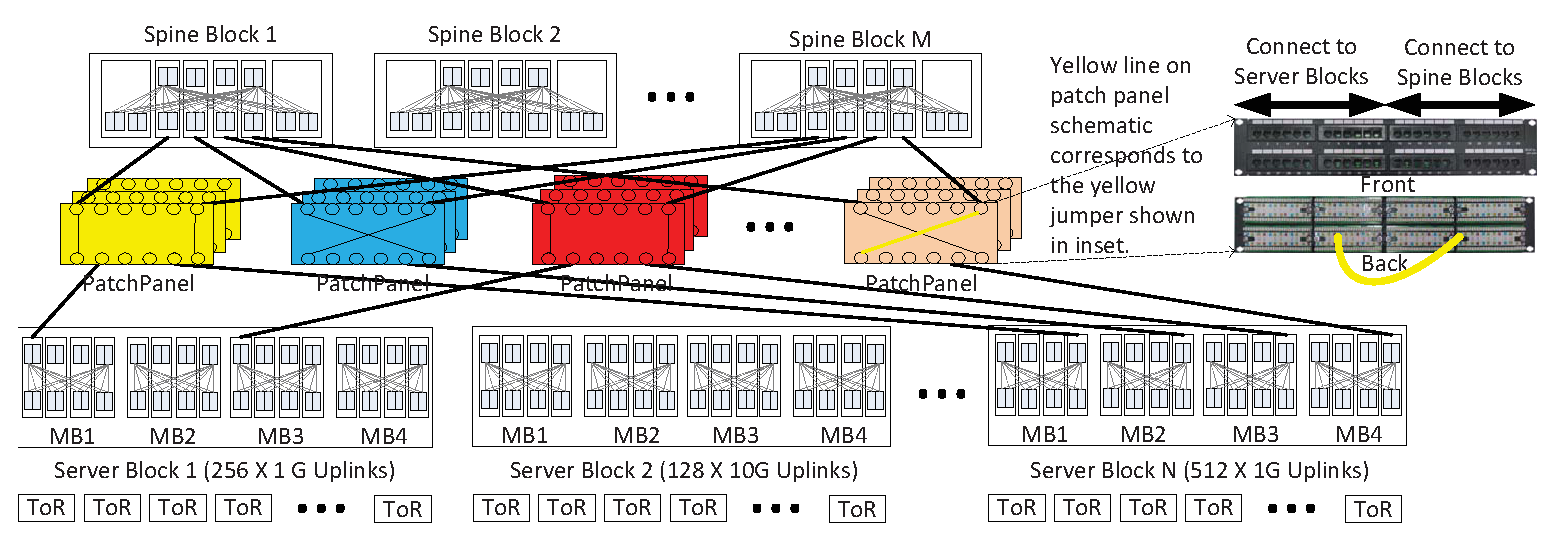
\includegraphics[scale=0.55]{topology}\\
\vspace{-1ex}
  \caption{Clos topology with a patch-panel layer, colored to indicate an example 4-stage expansion}
\label{topology}
\end{figure*}
\section{Prior Work on Expansions}

Prior work has described DCN designs that support incremental expansion, and techniques for conducting expansions. Our work focuses on Clos topologies, the de-facto standard for large-scale DCNs; most prior work on expansions has used non-Clos designs.

DCell~\cite{Dcell} and BCube~\cite{BCube} are built using iterative structures. As a result, they can only supports expansions at a very coarse granularity, which could lead to substantial stranded DCN capacity after expansion. Similar iteratively-designed DCN structures are also proposed in~\cite{ExpandableDcn2,FiConn,ExpandableDcn}.

JellyFish~\cite{Jellyfish}, Space Shuffle~\cite{SpaceShuffle}, Scafida~\cite{FreeScalingDcn}, and Expander~\cite{Xpander, ExpandingXpander} were designed to support fine-grained incremental expansion using random-graph-based DCN topologies. However, these topologies have not been widely adopted for industrial-scale data centers, possibly due to the increased complexity of cabling and routing and congestion control when deploying large-scale DCNs.

Random Folded Clos~\cite{RandomClos} is a variant of Clos that supports fine-grained incremental expansion. It maintains a layered structure, but builds inter-layer links based on random graphs. However, Random Folded Clos is only designed for homogeneous DCNs, where all blocks are of the same size and the same port speed. Further, Random Folded Clos is not non-blocking, with reduced capacity when compared to Fat Trees. In contrast, our minimal-rewiring solver can be applied to heterogeneous DCNs, and its topology solution preserves the non-blocking property of Clos topologies.

Similar to our minimal-rewiring DCN topology solver, optimization-based approaches were also adopted in LEGUP~\cite{LegUpDcn} and REWIRE~\cite{RewireDcn}. However, neither paper looked at the topology-design problem in the presence of a patch-panel layer, and could have daunting cabling complexity. Further, LEGUP uses a branch-and-bound algorithm~\cite{BranchAndBound}, and REWIRE uses simulated annealing~\cite{SimulatedAnnealing} to search for the optimal topology. Both algorithms scale poorly, as their convergence time grows exponentially with the problem size.

Condor~\cite{Condor} allowed designers to express goals for DCN topologies via a constraint-based language, and used a constraint solver to generate topologies.   Condor addressed the challenge of multi-phase expansions, but their approach was unable to solve expansions for many arbitrary configurations of Clos networks due to computational complexity.


\section{Overview of Clos-Based DCN Topology}
The Clos topology was initially designed for telephone networks~\cite{Clos}. Years later, it was proposed for DCNs~\cite{FatTree} and subsequently became the de-facto standard for large-scale DCNs, at Google~\cite{JupiterRising}, Facebook~\cite{FacebookDcn}, Cisco~\cite{CiscoDcn}, Microsoft~\cite{VL2}, etc.. There are many advantages to Clos networks. First, Clos networks are non-blocking, and thus have high throughput. Second, Clos networks can be built using identical and inexpensive commodity switches, and thus are cost-effective. Third, Clos networks have many of redundant paths for each source-destination pair, and thus are highly failure-resilient.

Clos-based data centers exhibit a layered architecture (see Fig.~\ref{topology}). The lower layer contains a number of \emph{server blocks}\footnote{``Server blocks'' are also called ``pods''~\cite{HybridDataCenter}, or ``edge aggregation blocks''~\cite{JupiterRising}.}.The upper layer contains a number of \emph{spine blocks}, used to forward traffic between server blocks. A DCN topology interconnects each server block to each spine block.  Because we want to support technology evolution within a single network, each of the server blocks could have a different number of spine-facing uplinks, a different uplink rate, etc\footnote{Fig.~\ref{topology} shows three server blocks with different uplink configurations.}.

Connecting server blocks and spine blocks by direct wires\footnote{We use the term ``wires'' to loosely refer to either fiber or copper links.} is highly inefficient. First,a large-scale data center typically has tens of thousands of DCN links. Second, the server blocks and the spine blocks of a data center may be deployed at different locations on a data center floor, due to space constraints, so some direct links would have to run a long way across the data center. Third, moving, adding, or removing a long link during an expansion requires significant human labor, creates a risk of error, and because the new links might have dramatically different lengths requires a large inventory of cables of various lengths.

To overcome these difficulties, we introduce a patch panel~\cite{PatchPanel, PatchPanelCabling} layer between server blocks and spine blocks (Fig. \ref{topology}). Patch panels are much cheaper than other DCN components (e.g., switches, optical transceivers, long-reach fibers). All the interconnecting ports of the server and spine blocks can be connected to the front side of the patch panels via fiber bundles, and all the connecting links can be established or changed using fiber jumpers on the back side\footnote{The inset photo in Fig. \ref{topology} depicts how we use these jumpers.  The yellow line on the right-most patch panel corresponds to the yellow jumper in the inset, which connects one server-block link to one spine-block link.}. These patch panels are co-located. As a result, a DCN topology can be wired and modified without walking around the data center floor or requiring the addition or removal of existing fiber.  Also, as discussed in~\cite{JupiterRising}, deploying fibers in bundles greatly reduces cost and complexity; using patch panels means we can deploy bundles once, without having to change them during an expansion. This patch-panel layer makes it much easier for us to support rapid expansions without excessive capacity reduction.

%\begin{figure}[ht]
 %\centering
 %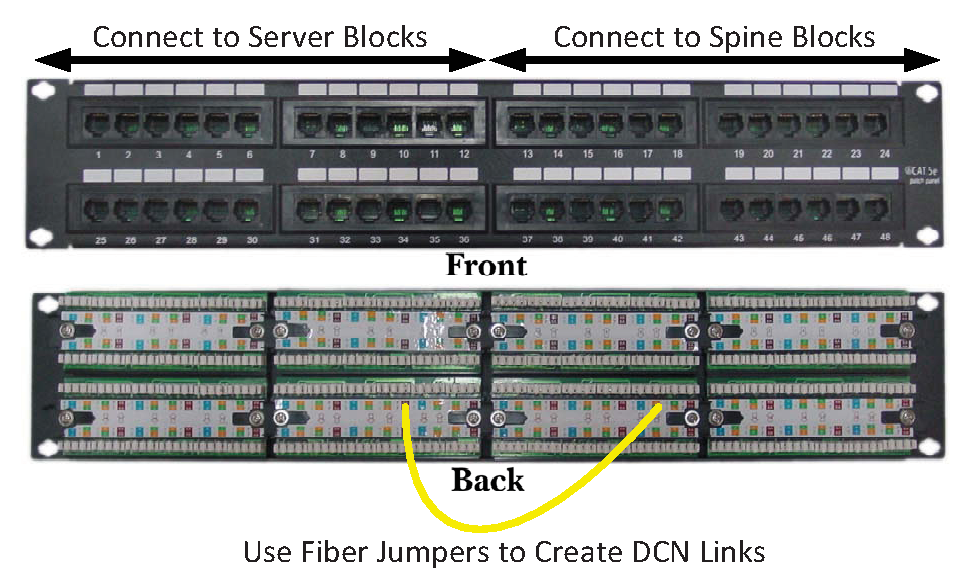
\includegraphics[scale=0.52]{patch_panel}\\
 %\caption{Use of patch-panel fiber jumpers to create DCN links}
%\label{patchpanel}
%\end{figure}

Patch panels allow us to divide a DCN topology into two layers, \emph{physical} and \emph{logical}. As shown in Fig. \ref{topology}, each server and spine block is connected to the patch-panel layer; we call this the \emph{physical topology}. When a new block is first deployed, we deploy its corresponding physical topology. Changing physical links is not easy, as it involves moving fiber bundles across different patch panels. Hence, in this paper, readers can view physical links as fixed once deployed. 

\emph{Logical topology} defines how server blocks connect to spine blocks, abstracting out the patch-panel layer.  All DCN topologies discussed in literatures refer to the logical topology. Many DCN performance metrics have been defined in terms of logical topologies, including network bandwidth, failure resiliency, incremental expandability, etc. 
However, except for Condor~\cite{Condor}, no prior work has studied the logical-topology design problem in presence of patch panels. 
As discussed in \S\ref{ConstraintsSection}, in addition to optimizing the performance metrics listed above, we also need to enforce additional physical constraints, so that the resulting logical topology is compatible with the underlying physical topology.

\subsection{Considerations for Clos expansions}

During an expansion, the existing physical topology remains unchanged, and we only add new bundles of physical links for the newly added/upgraded server/spine blocks. 
Note that adding new physical links does not impact any ongoing traffic. In contrast, some of the links in the existing logical topology, which could be carrying significant traffic, will have to change, so we must ensure there is no traffic loss caused by changes to the logical topology.

As shown in Fig. \ref{dcnstrandedcapacity} (a), we could add a large amount of capacity to a data center during each expansion, which would allow us to do expansions infrequently. However, this expansion strategy would lead to much more \emph{stranded} network capacity -- capacity installed but not usable -- as the traffic demand could be far less than the capacity provided.  By doing fine-grained expansions, we reduce the mean amount of stranded capacity (see Fig. \ref{dcnstrandedcapacity} (b)).
\begin{figure}[ht]
 \centering
 \subfigure[Coarse-Grained Expansion.]{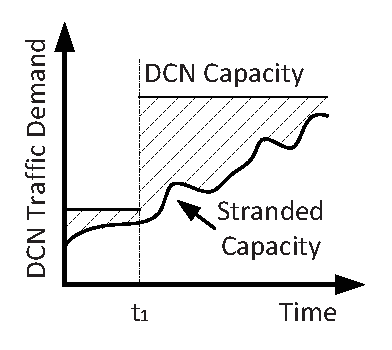
\includegraphics[scale=0.6]{coarse_expansion}}
 \subfigure[Fine-Grained Expansion.]{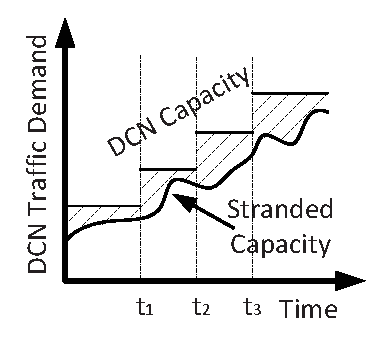
\includegraphics[scale=0.6]{fine_expansion}}
\vspace{-1ex}
 \caption{DCN stranded capacity.}\label{dcnstrandedcapacity}
\end{figure}\section{Patch-Panel Based Expansion Pipeline}
\label{PipelineSection}

\begin{comment} %% moved this to the previous section
To accommodate continuously-growing data center traffic demand, we must expand our data center networks regularly. As shown in Fig. \ref{dcnstrandedcapacity} (a), we could add a large amount of capacity to a data center during each expansion, which would allow us to do expansions infrequently. However, this expansion strategy would lead to much more \emph{stranded} network capacity -- capacity installed but not usable -- as the traffic demand could be far less than the capacity provided.  By doing fine-grained expansions, we reduce the mean amount of stranded capacity (see Fig. \ref{dcnstrandedcapacity} (b)).
\begin{figure}[ht]
 \centering
 \subfigure[Coarse-Grained Expansion.]{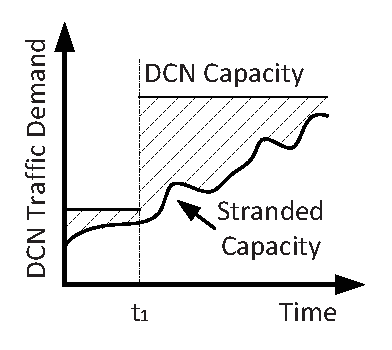
\includegraphics[scale=0.6]{coarse_expansion}}
 \subfigure[Fine-Grained Expansion.]{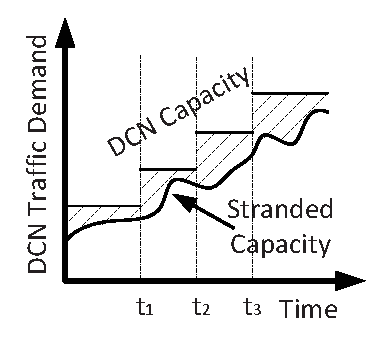
\includegraphics[scale=0.6]{fine_expansion}}
\vspace{-1ex}
 \caption{DCN Stranded Capacity.}\label{dcnstrandedcapacity}
\end{figure}
\end{comment}

We support two types of expansions, at the granularity of a server block (Fig. \ref{dcnexpansion}). The first type adds a new server block, to allow more servers to be added to an existing data center. The second type increases the uplink count (``radix'') of an existing server block. Typically, the uplinks of a server block are not initially fully populated with optical transceivers, because transceivers are expensive and a new server block has a low bandwidth requirement (as not all of its servers are connected). As a block's bandwidth requirement increases, we need to populate more uplinks. Note that as we expand the server-block layer, additional spine blocks will also be needed, so expansions generally involve adding server blocks and spine blocks at the same time.
\begin{figure}
 \centering
 \subfigure[Add a third server block]{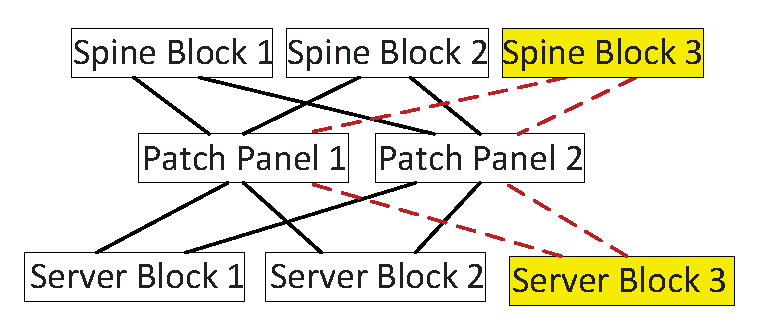
\includegraphics[scale=0.345]{expansion_new_sb}}
 \subfigure[Radix upgrade of a server block]{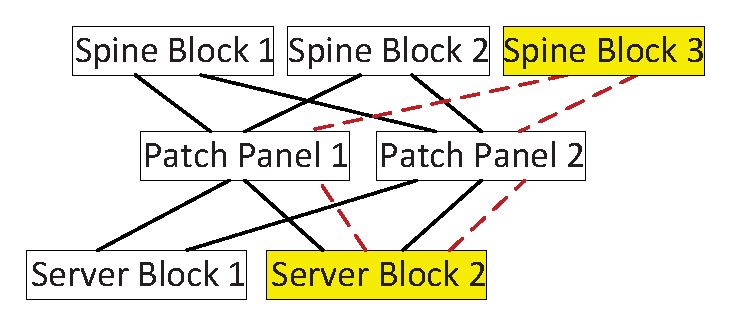
\includegraphics[scale=0.345]{expansion_radix_upgrade}}
\vspace{-1ex}
 \caption{Data center expansion types.}\label{dcnexpansion}
\end{figure}

Fig. \ref{expansionpipeline} depicts our pipeline for updating a logical topology during a live expansion.   It guarantees that:
\begin{MYitemize}
  \item No traffic loss due to routing packets into ``black holes.'' 
  \item All wiring changes are made correctly.
  \item No congestion due to the temporary capacity reduction.
\end{MYitemize}

\begin{figure}
 \centering
 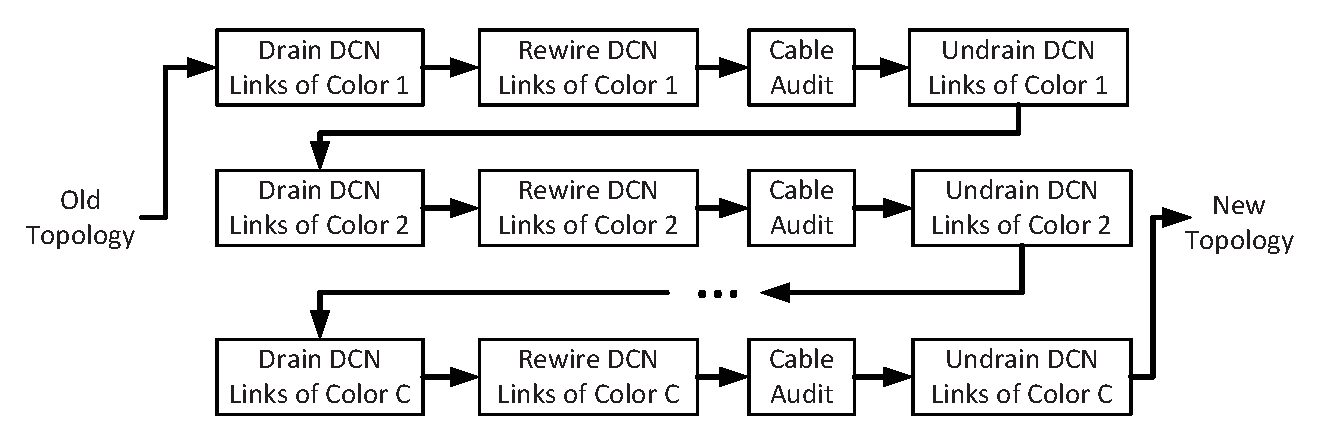
\includegraphics[scale=0.39]{pipeline}\\
\vspace{-1ex}
 \caption{DCN expansion pipeline.}\label{expansionpipeline}
\end{figure}

To avoid black holes when changing a set of logical links, we must redirect traffic on these links to other paths.  We instruct our SDN-based control plane to ``drain'' these links. After we verify that there is no longer traffic on the target drained links, we can proceed to rewire the links.

Rewiring links via patch-panel changes is the most labor-intensive and error-prone step. Typically, thousands of links need to be rewired during one expansion, creating the possibility of multiple physical mistakes during the rewiring process. To check for errors, we perform a \emph{cable audit}. In cable audit, we use the Link Layer Discovery Protocol to construct a post-wiring topology, and then cross-validate this against the target logical topology. We also run a bit-error-rate test (BERT) for all the new links, to detect links with issues.  This audit results in automated tickets to repair faulty links, followed by a repeat of the audit. 

During DCN expansion, we must drain some fraction of the logical links.  While Clos networks are resilient to some missing links, draining too many links simultaneously could result in dropping the network's available capacity below traffic demand.  We therefore set a residual-capacity threshold, based on measured demand plus some headroom.  We then divide an expansion into stages such that, during each stage, the residual capacity remains above this threshold.  In our original approach, we partitioned the set of patch panels into $C$ groups (as illustrated by different colors in Fig. \ref{topology}), and only rewired links in one group of patch panels per stage. Then, at each stage, we would still have approximately $1-1/C$ of the pre-expansion capacity available.

%% Figure deleted, per Amin’s advice that “I don't think that we need to show the growth rate
%% to motivate the importance of the problem” (and the numbers in this figure might not be
%% appropriate for external publication).
%\begin{figure}[ht]
 %\centering
 %% Requires \usepackage{graphicx}
 %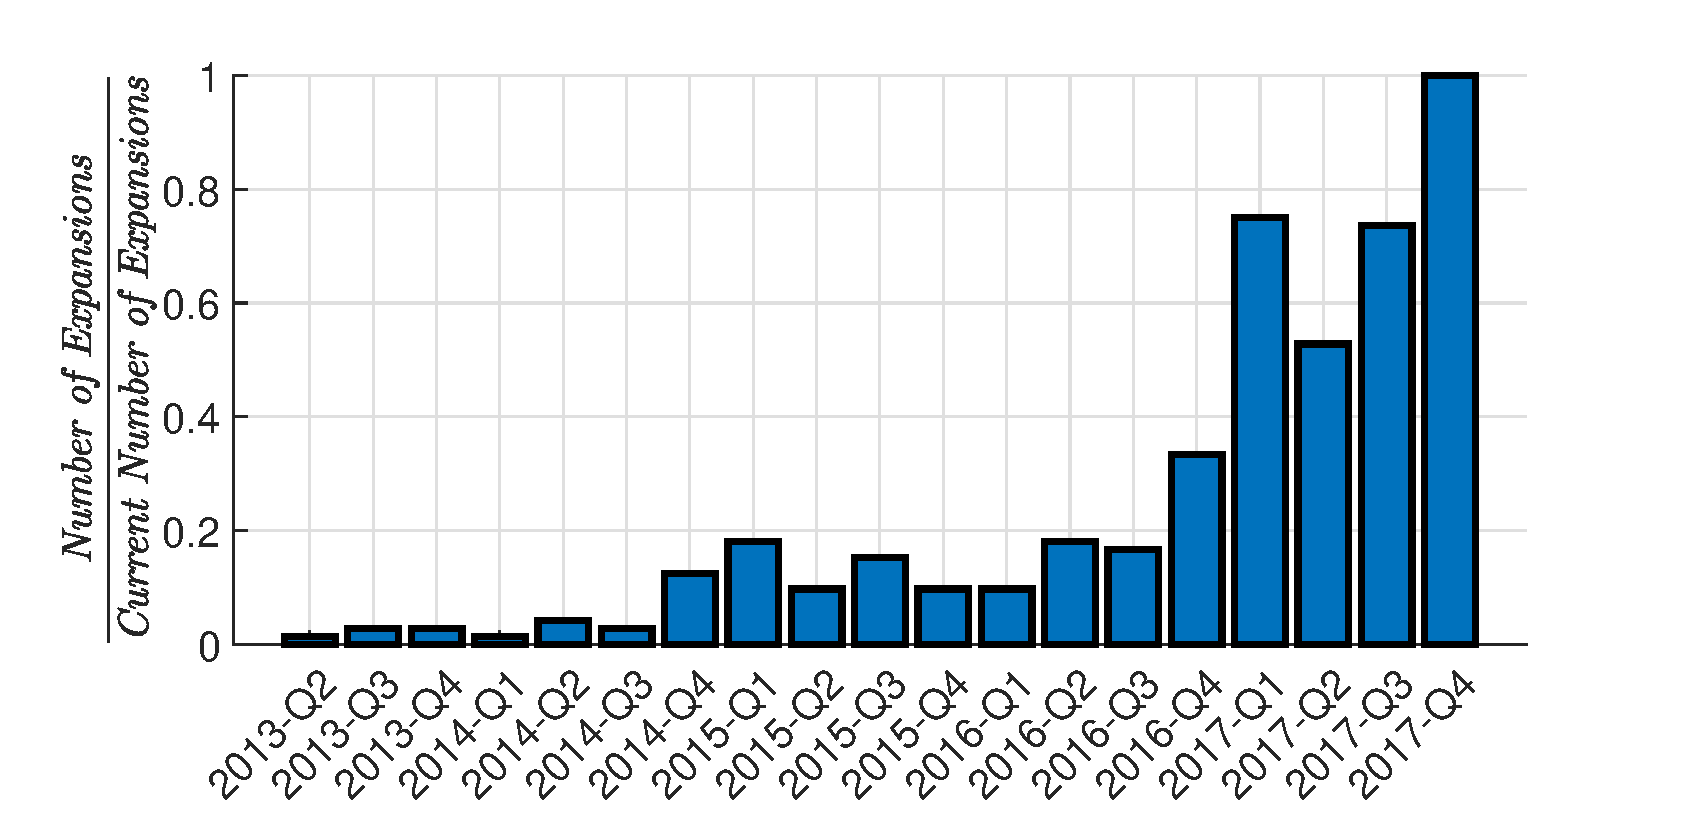
\includegraphics[scale=0.3]{num_expansions}\\
 %\caption{Total Number of Expansion Projects.}\label{numexpansions}
%end{figure}

Note that the expansion pipeline migrates the network, in stages, from an existing (old) topology to some new logical topology that connects the new blocks to the existing ones, subject to a set of constraints on the logical connectivity (\S\ref{ConstraintsSection} formalizes those constraints).  However, there are many ways to construct a logical topology that meets our constraints, and our original, simple solution to these constraints typically required a lot of rewiring for an expansion. This, in turn, forced us to divide expansions into $C$ stages, to ensure that we preserved at least $1-1/C$ of the pre-expansion capacity.  

As a result, these expansions took a long time, especially if the pre-expansion network was highly utilized.  In our experience, each stage takes considerable time, including draining, rewiring, cable auditing, BERTing, and undraining. If we were to expand a network with a requirement to preserve 90\% residual capacity, at least 10 stages would be needed\footnote{In fact, since failed links and inexact load balance can cause topology imperfections, more than 10 stages would be required to ensure 90\% residual capacity.}.
%As our workloads grows, the rate at which we must do expansions also grows, and these lengthy expansion timelines became unsustainable.

The root cause of the length of our original expansion pipeline is that it does not attempt to  optimize the difference (in terms of wiring changes) between pre-expansion and post-expansion topologies. If we were able to minimize this difference, we could finish an expansion in fewer stages. This is related to the ``incremental expansibility'' property of a DCN topology. This property is easy to achieve for random-graph topologies such as Jellyfish~\cite{Jellyfish}. However, for Clos networks, none of the existing topology solutions exhibits this property. This motivated us to look for a better approach, which we describe in the rest of this paper.
\section{Minimal Rewiring for DCN Expansion}
In this section, we describe a new ``minimal rewiring'' topology-design methodology for Clos networks, which not only achieves high network capacity and failure resiliency, but also minimizes rewiring for expansions. Our approach relies on Integer Linear Programming (ILP) to compute a logical topology. Our results compare well to existing Clos topology solutions \cite{JupiterRising,CiscoDcn,VL2,WCMP}.

While we initially considered an ILP formulation at the granularity of switch and patch-panel ports, the resulting scale made solving infeasible. Instead, we use multiple phases, first solving a block-level ILP formulation (\S\ref{ILPSection}) and then performing a straightforward mapping onto a port-level solution (\S\ref{MappingSection}).

\subsection{Definitions and notations}\label{DefinitionsSection}

To rigorously formulate the minimal-rewiring topology-design problem, we introduce the following definitions and mathematical notations.

\begin{table}[ht]
\small
\centering
\caption{Notations used in this paper}
\begin{tabular}{|c|p{2.4in}|}
\hline
$E_n$, $S_m$, $O_k$ & Server block $n$, spine block $m$, patch panel $k$\\
$E_n^t$ & Middle block $t$ in server block $n$ \\
\hline
$G_k(E_n^t) $ & Physical link-count for $E_n^t$ via patch panel $k$ \\
$G_k(S_m) $ & Physical link-count for $S_m$ via patch panel $k$ \\
$b_k(E_n^t, S_m)$ & Reference logical-topology link-count between $E_n^t$ and $S_m$ via patch panel $O_k$ \\
$d_k(E_n^t, S_m)$ & Desired logical-topology link-count between $E_n^t$ and $S_m$ via patch panel $O_k$ \\
\hline
$p_{n,m}$ & Mean number of links between a server block and a spine block \\
$q^t_{n,m}$ & Mean number of links between a middle block and a spine block \\
\hline
$n_g$ & Server block group index; or a set containing all the server block indices in the $n_g$-th group \\
$m_g$ & Spine block group index; or a set containing all the spine block indices in the $m_g$-th group \\
$k_g$ & Patch panel group index; or a set containing all the patch panel indices in the $k_g$-th group \\
\hline
$E_{n_g}$, $S_{m_g}$, $O_{k_g}$ & Server block group $n_g$, spine block group $m_g$, patch panel group $k_g$\\
$E_{n_g}^t$ & All the $t$-th middle blocks in $E_{n_g}$ \\
\hline
$b_{k_g}(E_{n_g}^t, S_{m_g})$ & Reference logical-topology link-count between $E_{n_g}^t$ and $S_{m_g}$ via patch panel group $O_{k_g}$ \\
$d_{k_g}(E_{n_g}^t, S_{m_g})$ & Desired logical-topology link-count between $E_{n_g}^t$ and $S_{m_g}$ via patch panel group $O_{k_g}$ \\
\hline
$x^+$ & $\max\{0,x\}$ \\
%$\lceil x \rceil$ & The smallest integer that is no smaller than $x$ \\
%$\lfloor x \rfloor$ & The largest integer that is no larger than $x$ \\
\hline
\end{tabular}
\label{notations}
\end{table}

\paragraph{Server Block:} We use a server block as a unit of deploying network-switching capacity.  On the order of 1000 servers can be connected to a server block via ToR switches. To avoid a single point of failure, we further divide a server block into  independent \emph{middle blocks}, typically four \footnote{Our results hold for any number of middle blocks.}  (see Fig. \ref{topology}); each middle block is controlled by a different routing controller. The uplinks of each ToR switch are evenly spread among the middle blocks in its server block. Even if one middle block is down, servers in the server block are still accessible via its other middle blocks. We assume that a DCN has  $N$ server blocks, each of which is represented by $E_n, n=1,2,...,N$. We denote the middle blocks within server block $E_n$ by $E_n^t, t=1,2,3,4$.

\paragraph{Spine Block:} Spine blocks forward traffic among different server blocks. We use $S_m, m=1,2,...,M$ to represent a spine block, where $M$ is the total number of spine blocks.

\paragraph{Physical Topology:}  Assume there are $K$ patch panels, each of which is represented by $O_k, k=1,2,...,K$. We use $G_k(E_n^t)$ to represent the total number of physical links between the middle block $E_n^t$ and the patch panel $O_k$. Then, the physical topology of server block $E_n$ can be characterized by $\{G_k(E_n^t), k=1,...,K, t=1,2,3,4\}$\footnote{Here we use the term ``topology'' somewhat loosely to describe the cardinality of the connectivity between a block and a set of patch panels, rather than to describe either the detailed inter-block topology, or the internal topology within a block composed of multiple commodity switches.}. 

Similarly, we use $G_k(S_m)$ to represent the total number of physical links between spine block $S_m$ and patch panel $O_k$. Then, the physical topology of spine block $S_m$ can be characterized by $\{G_k(S_m), k=1,...,K\}$. 

Note that our networks are heterogeneous: different server blocks and spine blocks could have different physical topologies (see Table \ref{blocktypes} for details).

\paragraph{Reference Topology:} Our goal is to minimize rewiring with respect to the old logical topology, called the \emph{reference topology}. We let $b_k(E_n^t, S_m)$ be the total number of reference-topology links between middle block $E_n^t$ and spine block $S_m$ that connect via patch panel $O_k$. Since the new server and spine blocks do not exist in the reference topology, for these blocks we simply set $b_k(E_n^t, S_m) = 0$.

\paragraph{Logical Topology:} Our objective is to compute a new logical topology for the given physical topology. We use $d_k(E_n^t, S_m)$ to represent the total number of logical links between middle block $E_n^t$ and spine block $S_m$ that connect via patch panel $O_k$. As we will show shortly, as long as $\{d_k(E_n^t, S_m)\}_{k,m,n,t}$ satisfies a set of physical topology constraints, a polynomial-time algorithm can be used to map  $\{d_k(E_n^t, S_m)\}_{k,m,n,t}$ to point-to-point configurations in the patch panels. Hence, the objective of the block-level ILP formulation is to compute $\{d_k(E_n^t, S_m)\}_{k,m,n,t}$.


\subsection{ILP Formulation of Minimal Rewiring}\label{ILPSection}

Our ILP formulation consists of a set of constraints (\S\ref{ConstraintsSection}) and an objective (\S\ref{ObjectiveSection}).

\subsubsection{Constraints for Logical Topology}\label{ConstraintsSection}

Recall that our objective is to compute $\{d_k(E_n^t, S_m)\}_{k,m,n,t}$.  We must impose a set of constraints on the solution, not only to ensure the compatibility of the logical topology with the underlying physical topology, but also to guarantee both high throughput and high failure resiliency.


\paragraph{Physical Topology Constraints:}
Recall that $d_k(E_n^t, S_m)$ is the total number of logical links between middle block $E_n^t$ and spine block $S_m$ connected via patch panel $O_k$. Clearly, it must be no larger than the total number of physical links $G_k(E_n^t)$ between $O_k$ and $E_n^t$, and the total number of physical links $G_k(S_m)$ between $O_k$ and $S_m$, i.e.,
\begin{equation}\label{blockdecisionvariables}
0\leq d_k(E_n^t, S_m)\leq\min\{G_k(E_n^t), G_k(S_m)\}.
\end{equation}

To ensure high uplink bandwidth for all the server blocks, we require that each ``populated'' server block port\footnote{Recall that, for cost reasons, we do not initially populate all the ports.} must connect to a spine block port. 
This is guaranteed by
\begin{equation}\label{superblockconnect}
\sum_{m=1}^M d_k(E_n^t, S_m)=G_k(E_n^t).
\end{equation}

Note that constraint (\ref{superblockconnect}) requires that the total number of spine block ports must be no smaller than the total number of server block ports on each patch panel. Hence, it is possible that a physically-connected spine block port might not connect to any server block port, which can be expressed as:
\begin{equation}\label{spineblockconnect}
\sum_{n=1}^N\sum_{t=1}^4 d_k(E_n^t, S_m)\leq G_k(S_m).
\end{equation}

\paragraph{Capacity Constraints:}
In order to achieve high DCN capacity, which depends on load balance, we require the uplinks of each server block to be evenly distributed among all spine blocks. Specifically,
\begin{equation}\label{superspineblockconstraint}
\lfloor p_{n,m}\rfloor\leq \sum_{k=1}^K\sum_{t=1}^4 d_k(E_n^t, S_m)\leq \lceil p_{n,m}\rceil,
\end{equation}
where $p_{n,m}$ is the mean number of links between a server block and a spine block.
$p_{n,m}=|E_n||S_m|/(|S_1|+\cdots+|S_M|)$\footnote{We have assumed,  when deriving $p_{n,m}$,  that the number of spine block ports is no less than the number of server block ports. In fact, our formulation and the subsequent optimization techniques also apply to the cases where there are fewer spine block ports.}, where $|E_n|$ (or $|S_m|$) is the total number of ports in $E_n$ (or $S_m$), $\lfloor p_{n,m}\rfloor$ is the largest integer that is no larger than $p_{n,m}$, and $\lceil p_{n,m}\rceil$ is the smallest integer that is no smaller than $p_{n,m}$.

Constraint (\ref{superspineblockconstraint}) ensures high DCN capacity. In the ideal case where all $p_{n,m}$'s are integers, constraint (\ref{superspineblockconstraint}) ensures that traffic between any two server blocks $E_{n_1}$ and $E_{n_2}$ can burst at full rate ($\min\{|E_{n_1}|, |E_{n_2}|\}$). Specifically, $E_{n_1}$ and $E_{n_2}$ can communicate at rate $\min\{p_{n_1,m}, p_{n_2,m}\}$ through the $m$-th spine block, and thus the total rate would be $\sum_{m=1}^M\min\{p_{n_1,m}, p_{n_2,m}\}=\min\{|E_{n_1}|, |E_{n_2}|\}$.

In the general case where some $p_{n,m}$'s are not integers, there must be some imbalance in the logical topology. Constraint (\ref{superspineblockconstraint}) minimizes this imbalance.

%As readers will see in Section \ref{throughputanalysis}, DCNs satisfying Constraint (\ref{superspineblockconstraint}) achieve $>97\%$ of the optimal throughput for permutation traffic pattern, and $>99\%$ of the optimal throughput for uniform traffic pattern, on average.

\paragraph{Failure-Resiliency Constraints:}
% This sentence cites DcnFailures in a confusing way (the most obvious parsing is not
% actually supported by that paper).
%As reported in \cite{DcnFailures}, commodity switches are highly reliable, and most data
% center failures happen in middle blocks\footnote{Middle block is referred to as aggregation
%switch in \cite{DcnFailures}.} due to software problems in the controllers. 
While commodity switches are highly reliable, an entire middle block can fail as a unit due to software bugs in its routing controller. We also bring down an entire middle block occasionally to upgrade the switch stack softwares. In order for our DCN to be failure-resilient, we need to make sure that throughput remains as high as possible even under middle-block failures. This can be achieved by requiring the middle block links to be evenly distributed among the spine blocks. Specifically,
\begin{equation}\label{middlespineblockconstraint}
\lfloor q^t_{n,m}\rfloor\leq \sum_{k=1}^K d_k(E_n^t, S_m)\leq \lceil q^t_{n,m}\rceil,
\end{equation}
where $q^t_{n,m}$ is the mean number of links between a middle block and a spine block\footnote{Our formulas for $p$ and $q$ require trivial extensions to support heterogeneous link speeds; we omit these for reasons of space.}.
$q^t_{n,m}=|E^t_n||S_m|/(|S_1|+\cdots+|S_M|)=p_{n,m}/4$ (assuming $4$ middle blocks per server block).

Constraint (\ref{middlespineblockconstraint}) minimizes the capacity impact under middle block failures. In the ideal case where $q^t_{n,m}$'s are all integers, the throughput impact is exactly 25\%. In the general case where some $q^t_{n,m}$'s are not integers, there must be some imbalance in the traffic between the middle blocks and the spine blocks. Constraint (\ref{middlespineblockconstraint}) minimizes this imbalance. Note that Constraint (\ref{middlespineblockconstraint}) cannot subsume (\ref{superspineblockconstraint}), because all the decision variables are integers.

%We also simulate a large number of realistic scenarios in Section \ref{throughputanalysis}. Under middle block failures, DCNs satisfying Constraint (\ref{middlespineblockconstraint}) still achieve $>74\%$ of the optimal throughput for permutation traffic pattern, and $>70\%$ of the optimal throughput for uniform traffic pattern, on average.

\subsubsection{Minimal-Rewiring ILP Objective}\label{ObjectiveSection}

In our ILP-based formulation, it is easy to add a minimal-rewiring objective function. Specifically,  our block-level minimal-rewiring solver can be formulated as:
\begin{eqnarray}\label{blocklevelminimalrewiring}
&\min&\sum_{k=1}^K\sum_{n=1}^N\sum_{t=1}^4\sum_{m=1}^M(b_k(E_n^t,S_m)-d_k(E_n^t,S_m))^+, \nonumber\\
&\text{subject to}&(\ref{blockdecisionvariables})-(\ref{middlespineblockconstraint}),
\end{eqnarray}
where $x^+=\max\{0,x\}$. This objective function computes the total number of links to be rewired for changing the old (reference) topology to the new topology.

\subsection{Benefits of Minimal Rewiring}\label{MRbenefitSection}
We demonstrate the benefit of minimal rewiring using a simple example, comparing our minimal-rewiring approach against the \emph{rotation striping} approach described in~\cite{WCMP}. Rotation striping can be used to design Clos topologies for \emph{homogeneous} DCNs of arbitrary size,whereas minimal-rewiring works with various block sizes.

Consider a DCN configuration with $N$ server blocks and  $M$ spine blocks. Assume that each server block has $X$ ports, and that there is only one patch panel\footnote{Rotation striping does not consider the patch-panel layer, which is equivalent to setting the number of patch panels to be 1.}. Then, rotation striping can be expressed as Algorithm \ref{RotationStriping}.

\begin{algorithm}
\small
\KwIn{DCN configuration parameters $N$, $M$, $X$}
\KwOut{A DCN topology}
Label all the server block ports with different indices from $1, 2,..., NX$. Note that the set of ports $\{(n-1)X+1, (n-1)X+2, ..., nX\}$ corresponds to the $n$-th server block.

Connect port $e\in \{1, 2,..., NX\}$ to the $\lceil e/M\rceil$-th port of the $((e-1)\%M + 1)$-th spine block.
\caption{Rotation striping algorithm from ~\cite{WCMP}}\label{RotationStriping}
\end{algorithm}

We can quantify the \emph{rewiring ratio} for a solution as the fraction of wires between server blocks and spine blocks in the pre-existing topology that must be disconnected during an expansion procedure.

Consider an expansion in which we add $1$ server block and $1$ spine block. It is easy to check that with rotation striping, only the first $M$ server-block ports connect to their original peers, and thus the rewiring ratio would be $(NX-M)/NX$.

On the other hand, using minimal-rewiring\footnote{Rotation striping can only guarantee the constraints (\ref{blockdecisionvariables})-(\ref{superspineblockconstraint}). Hence, \emph{for this example}, we also only impose those constraints on our minimal rewiring solver.}, we can show that only $XN/(M+1)$ links need to be rewired, which corresponds to a rewiring ratio of $1/(M+1)$. This means that even if our expansion is executed in just a single stage, the capacity reduction is just $1/(M+1)$.


% I think the next 3 paragraphs are mostly still about the benefits of mimimal-rewiring,
% not the challenges
To the best of our knowledge, with the exception of Condor~\cite{Condor}, none of the prior literature has incorporated patch-panel layer constraints, and Condor's constraint-satisfaction approach was unable to find solutions in most cases. In practice, we usually need more than one patch panels in order to connect all the server blocks to all the spine blocks, since the number of ports on each patch panel is limited. If one ignores the patch-panel layer, then the resulting DCN topology will be very likely not compatible with the underlying physical topology.

Consider rotation striping in an example with two patch panels (see Fig. \ref{infeasible}). Each server block has six links, with three links connecting to the first patch panel and the other three connecting to the second one. There are four spine blocks, with two of them connecting to the first patch panel and the other two connecting to the second one. If we apply rotation striping here, there should be four logical links between the first server block and the first two spine blocks. Note that these four links can only be created through the first patch panel, because the first two spine blocks only connect to the first patch panel. However, this is impossible, as there are only three physical links between the first server block and the first patch panel.
\begin{figure}[ht]
 \centering
 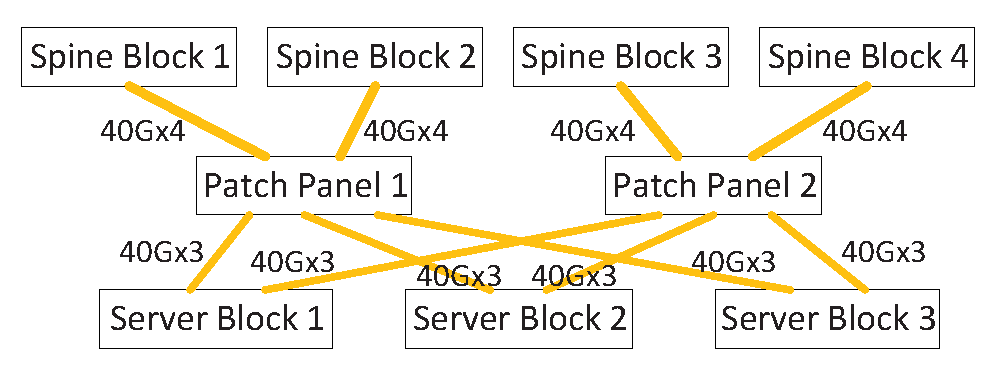
\includegraphics[scale=0.40]{infeasible}\\
\vspace{-1ex}
 \caption{A counterexample for which rotation striping fails.}\label{infeasible}
\end{figure}

Our approach incorporates the patch-panel layer via three physical constraints (\ref{blockdecisionvariables})-(\ref{spineblockconnect}). These three constraints ensure that any solution $\{d^*_k(E_n^t,S_m)\}_{k,m,n,t}$ of (\ref{blocklevelminimalrewiring}) can be mapped to port-to-port configurations in the patch panels as we describe below.  (Note that (\ref{blocklevelminimalrewiring}) may yield multiple solutions.)

\subsection{Creating port-to-port mappings}\label{MappingSection}


Our ILP formulation tells us the block-level link count  between each middle block $E_n^t$ and each spine block $S_m$ in each patch panel $O_k$, as in (\ref{blocklevelminimalrewiring}), but not how individual ports must be connected. We thus developed 
%Algorithm \ref{2pass} 
a straightforward algorithm to compute these port-to-port mappings.

The algorithm's input consists of the block-level link counts $b_k(E_n^t,S_m)$ and $d^*_k(E_n^t,S_m)$ for the pre-expansion and post-expansion topologies, respectively.  We use two passes, both of which iterate over all pairs of middle blocks and spine blocks:

\textbf{Pass 1: disconnect links as necessary:}
For each patch panel $O_k$, note that an expansion changes the link count between middle block $E_n^t$ and spine block $S_m$ from  $b_k(E_n^t,S_m)$ to $d^*_k(E_n^t,S_m)$.  Therefore, if $b_k(E_n^t,S_m)$ $\leq d^*_k(E_n^t,S_m)$, we simply preserve all pre-existing links; if $b_k(E_n^t,S_m)>d^*_k(E_n^t,S_m)$, we can disconnect any $(b_k(E_n^t,S_m)$ $-d^*_k(E_n^t,S_m))$ of the pre-existing links. This pass disconnects $\sum_{n=1}^N\sum_{t=1}^4\sum_{m=1}^M(b_k(E_n^t,S_m)-d^*_k(E_n^t,S_m))^+$ links.

\textbf{Pass 2: connect new links:}
After the first pass, $\min\{b_k(E_n^t,S_m), d^*_k(E_n^t,S_m)\}$ links remain between
$E_n^t$ and $S_m$.  For any block pair $E_n^t$ and $S_m$ with less than $d^*_k(E_n^t,S_m)$ links, we can arbitrarily pick $d^*_k(E_n^t,S_m)-b_k(E_n^t,S_m)$ non-connected ports from $E_n^t$ and $S_m$ respectively, and interconnect them. Feasibility is guaranteed by the physical topology constraints (\ref{blockdecisionvariables})-(\ref{spineblockconnect}).

\begin{comment}
In Algorithm \ref{2pass}, $e$  represents a server-block-facing patch-panel port in $O_k$, and $s$ represents a spine-block-facing patch-panel port in $O_k$. $e\in E_n^t, s\in S_m$ means that $e$ is connected to $E_n^t$, and $s$ is connected to $S_m$. $d^*(e,s)=1$ means a fiber jumper is used to connect $e$ and $s$ in patch panel $O_k$. 

In Algorithm \ref{2pass}, all block pairs $(E_n^t, S_m)$ are traversed twice. In the first pass, we disconnect all the old logical links that require rewiring. Specifically, for every block pair $(E_n^t, S_m)$, exactly $(b_k(E_n^t,S_m)-d^*_k(E_n^t,S_m))^+$ links are removed, at line 6. Thus, the total number of rewires for all the patch panels would be exactly $\sum_{k=1}^K\sum_{n=1}^N\sum_{t=1}^4\sum_{m=1}^M(b_k(E_n^t,S_m)-d^*_k(E_n^t,S_m))^+$. In the second pass, we establish the new logical links. Note that we need to find $(d^*_k(E_n^t,S_m)-b_k(E_n^t,S_m))$ unconnected ports from $E_n^t$ and $S_m$, respectively, in the \textbf{for} loop at lines 11-13. Feasibility is guaranteed by the physical topology constraints (\ref{blockdecisionvariables})-(\ref{spineblockconnect}).
\end{comment}

\begin{comment}
\begin{algorithm}[ht]
\small
\KwIn{A fixed patch panel $O_k$, and a solution $\{d^*_k(E_n^t,S_m)\}_{m,n,t}$ in $O_k$}
\KwOut{A port-to-port configuration $d^*(e,s)$ in $O_k$}
   Initialize $d^*(e,s) = 0$ for all the $(e,s)$ pairs.

   \For {any middle block $E_n^t$ and spine block $S_m$} {
     \uIf {$d^*_k(E_n^t, S_m) \geq b_k(E_n^t, S_m)$} {
       Set $d^*(e,s) = 1$ whenever $b(e,s) = 1$, for all the $e\in E_n^t$ and $s\in S_m$\;
     }
     \Else {
       Choose any $d^*_k(E_n^t, S_m)$ number of $(e,s)_{e\in E_n^t, s\in S_m}$ pairs in $O_k$ whose $b(e,s)=1$, and set $d^*(e,s) = 1$ for the chosen $(e,s)$ pairs\;
     }
   }
   \For {any middle block $E_n^t$ and spine block $S_m$} {
     \If {$d^*_k(E_n^t, S_m) > b_k(E_n^t, S_m)$} {
       \For {$i = 1$ to $d^*_k(E_n^t, S_m)-b_k(E_n^t, S_m)$} {
         Choose two unconnected ports $e\in E_n^t$ and $s\in S_m$ in the $k$-th patch panel arbitrarily, and set $d^*(e,s) = 1$.
       }
     }
   }
TODO(mogul@): more space at left margin for line numbers
\caption{Two-Pass Algorithm.}\label{2pass}
\end{algorithm}
\end{comment}

\subsection{Challenge: Solver Scalability}
We use integer linear programming to formulate our minimal-rewiring solver, because our topology-design problem is NP-Complete. Specifically, the decision variables $d_k(E_n^t,S_m)$ contain three dimensions (middle-block dimension $E_n^t$, spine-block dimension $S_m$, and patch-panel dimension $k$ ), and the constraints (\ref{superblockconnect})(\ref{spineblockconnect})(\ref{middlespineblockconstraint}) are essentially for the 2-marginal sums $\sum_k d_k(E_n^t,S_m)$, $\sum_{E_n^t} d_k(E_n^t,S_m)$ and $\sum_{S_m} d_k(E_n^t,S_m)$. In the literature, this is called the Three-Dimensional Contingency Table (3DCT) problem, and has been proven to be NP-Complete \cite{3DCT}. Having failed to find a polynomial-time algorithm for our problem, we decided to use ILP, as there are many readily-available commercial ILP solvers, e.g., Gurobi \cite{Gurobi}, {\ifpaper \else CPLEX \cite{CPLEX}, \fi} Google Optimization Tools \cite{GoogleOrTool}.

%However, our problem size is so large that none of the existing commercial solvers scales well. For example, one DCN configuration we simulate contains 30 Type-1, 20 Type-2, 27 Type-3 server blocks and 16 Type-1, 52 Type-2 spine blocks (see \S\ref{dcn_configurations}). Without any optimization, the total number of decision variables is about 400000. The ILP solver kept running for a day without generating a solution.As readers will see in \S\ref{solverrunningtimesection}, for all the 4500 DCN configurations, only 32\% of them can be solved in a 3-hour time limit. 
%\emph{TODO(mogul@): we should update these numbers to match the evaluation section}

However, our problem size is so large that none of the existing commercial solvers scales well. For example, one DCN configuration we evaluate (see \S\ref{concrete_example}) contains 77 server blocks of three kinds, 68 spine blocks of two kinds, and 256 patch panels. Without any optimization, this leads to about 400000 decision variables, and the ILP solver ran for a day without generating a solution.  As shown in \S\ref{solverrunningtimesection}, for the 4500 trials we ran without optimization, we could only solve 32\% within a 3-hour deadline. (Longer timeouts yield little improvement.)

\section{Block Aggregation}
To improve the scalability of our minimal-rewiring solver, we developed a block aggregation technique. Block aggregation significantly reduces the total number of decision variables in (\ref{blocklevelminimalrewiring}), and thus greatly improves solver scalability.

\subsection{ILP Formulation with Block Aggregation}
The idea behind block aggregation is to group patch panels, server blocks, spine blocks, and then aggregate decision variables within each group.

{\bf Patch-Panel Group:} Two patch panels $k_1, k_2$ belong to the same group if and only if they have the same number of physical links to each middle block and each spine block, i.e., $G_{k_1}(E_n^t) = G_{k_2}(E_n^t), G_{k_1}(S_m) = G_{k_2}(S_m)$ for any $n, t, m$.

{\bf Server-Block Group:} Two server blocks $n_1, n_2$ belong to the same group if and only if they have the same physical topology, i.e., $G_k(E_{n_1}^t) = G_k(E_{n_2}^t)$ for any $k, t$.

{\bf Spine-Block Group:} Two spine blocks $m_1, m_2$ belong to the same group if and only if they have the same physical topology, i.e., $G_k(S_{m_1}) = G_k(S_{m_2})$ for any $k$.

Assume that these definitions yield $K_g$ patch-panel groups, $N_g$ server-block groups, and $M_g$ spine-block groups. Then, we can define an aggregated decision variable $d_{k_g}(E_{n_g}^t, S_{m_g})$ for the $k_g$-th patch-panel group, the $n_g$-th server block group, and the $m_g$-th spine block group as follows:
\begin{equation}\label{aggregatedvariables}
d_{k_g}(E_{n_g}^t, S_{m_g})=\sum_{k\in k_g}\sum_{n\in n_g}\sum_{m\in m_g}d_k(E_n^t, S_m).
\end{equation}
Here, we have abused the notation, and used $k_g, n_g$, and $m_g$ to represent both the indices and the actual groups.

With the aggregated decision variables $d_{k_g}(E_{n_g}^t, S_{m_g})$, the original constraints (\ref{blockdecisionvariables})-(\ref{middlespineblockconstraint}) also need to be aggregated:
\begin{equation}\label{blockaggregateblockdecisionvariables}
0\leq d_{k_g}(E_{n_g}^t, S_{m_g})\leq |k_g||n_g||m_g|\min\{G_k(E_n^t), G_k(S_m)\},
\end{equation}
\begin{equation}\label{blockaggregatesuperblockconnect}
\sum_{m_g=1}^{M_g}d_{k_g}(E_{n_g}^t, S_{m_g}) = |k_g||n_g|G_k(E_n^t),
\end{equation}
\begin{equation}\label{blockaggregatespineblockconnect}
\sum_{n_g=1}^{N_g}\sum_{t=1}^4d_{k_g}(E_{n_g}^t, S_{m_g}) \leq |k_g||m_g|G_k(S_m),
\end{equation}
\begin{equation}\label{blockaggregatesuperspineblockconstraint}
|n_g||m_g|\lfloor p_{n,m}\rfloor\leq \sum_{k_g=1}^{K_g}\sum_{t=1}^4 d_{k_g}(E_{n_g}^t, S_{m_g})\leq |n_g||m_g|\lceil p_{n,m}\rceil,
\end{equation}
\begin{equation}\label{blockaggregatemiddlespineblockconstraint}
|n_g||m_g|\lfloor q^t_{n,m}\rfloor\leq \sum_{k_g=1}^{K_g}d_{k_g}(E_{n_g}^t, S_{m_g})\leq |n_g||m_g|\lceil q^t_{n,m}\rceil.
\end{equation}
In the aggregated  constraints, $k, n, m$ are arbitrary patch panel, server block, and spine block indices, drawn from the $k_g$-th patch-panel group, the $n_g$-th server-block group, and the $M_g$-th spine-block group, respectively. In fact, the values $G_k(E_n^t)$, $G_k(S_m), p_{n,m}, q^t_{n,m}$ are all the same, as long as $k, n, m$ are chosen in the same group, respectively. Here, we also view $k_g, n_g$, and $m_g$ as groups, and have used $|k_g|, |n_g|, |m_g|$ to represent the sizes of these groups.

With block aggregation, we can thus rewrite the optimization problem (\ref{blocklevelminimalrewiring}) as follows:
\begin{eqnarray}\label{minimalrewiringwithblockaggregation}
&&\hspace{-18mm}\min\hspace{1mm}\sum_{k_g=1}^{K_g}\sum_{n_g=1}^{N_g}\sum_{t=1}^4\sum_{m_g=1}^{M_g}(b_{k_g}(E_{n_g}^t, S_{m_g}) - d_{k_g}(E_{n_g}^t, S_{m_g}))^+, \nonumber\\
&\text{subject to}&(\ref{blockaggregateblockdecisionvariables})-(\ref{blockaggregatemiddlespineblockconstraint}),
\end{eqnarray}
where $b_{k_g}(E_{n_g}^t, S_{m_g})=\sum_{k\in k_g}\sum_{n\in n_g}\sum_{m\in m_g}b_k(E_n^t, S_m)$.

Compared to (\ref{blocklevelminimalrewiring}), the total number of decision variables in (\ref{minimalrewiringwithblockaggregation}) is significantly reduced, from $\Theta(NKM)$ to $\Theta(N_gK_gM_g)$. Thus, the complexity of solving (\ref{minimalrewiringwithblockaggregation}) is significantly lower than that of (\ref{blocklevelminimalrewiring}).

\subsection{Variable Deaggregation}
After obtaining a solution $d^*_{k_g}(E_{n_g}^t, S_{m_g})$ for (\ref{minimalrewiringwithblockaggregation}), we still need to decompose the solution to $d^*_{k}(E_{n}^t, S_{m})$. Specifically, we need to solve the following problem.
\begin{eqnarray}\label{mrstep2}
&\min&\sum_{k=1}^K\sum_{n=1}^N\sum_{t=1}^4\sum_{m=1}^M(b_k(E_n^t,S_m)-d_k(E_n^t,S_m))^+,\nonumber\\
&\text{subject to}& \sum_{k\in k_g}\sum_{n\in n_g}\sum_{m\in m_g}d_k(E_n^t, S_m)=d^*_{k_g}(E_{n_g}^t, S_{m_g})\nonumber\\
&&\text{and }(\ref{blockdecisionvariables})-(\ref{middlespineblockconstraint}).
\end{eqnarray}

If there were no constraints (\ref{blockdecisionvariables})-(\ref{middlespineblockconstraint}) in (\ref{mrstep2}), we could easily compute a solution $d^*_{k}(E_{n}^t, S_{m})$ in polynomial time using an algorithm similar to the one in \S\ref{MappingSection}.
%Algorithm \ref{2pass}. 
Because of these constraints, solving (\ref{mrstep2}) becomes much more challenging. In fact, it is not trivial to prove that (\ref{mrstep2}) always has a solution. In the literature, (\ref{mrstep2}) is closely related to the Integer-Decomposition property~\cite{IntegerDecomposition}. In general, the Integer-Decomposition property does not always hold 
\ifpaper (an example is provided in~\cite{TechnicalReport}).
\else (see Appendix \ref{CounterExample}).
\fi
 Fortunately, thanks to our problem structure, we are able to rigorously prove that (\ref{mrstep2}) indeed has a solution. Specifically, we build an integer decomposition theory specifically for our problem, and prove that a decomposition satisfying (\ref{blockdecisionvariables})-(\ref{middlespineblockconstraint}) can be found iteratively in polynomial time. 
\ifpaper The details are available in~\cite{TechnicalReport}.
\else (See the Appendices for details.)
\fi

Given that (\ref{mrstep2}) has solutions, the next question is to find one that minimizes the objective function. The simplest approach is to directly solve it using integer programming. However, this will destroy the complexity-reduction of block aggregation, as (\ref{mrstep2}) is of exactly the same size as (\ref{blocklevelminimalrewiring}).

Our approach is to decompose (\ref{mrstep2}) into $K_g+N_g+M_g$ smaller ILP problems. Specifically, we can decompose patch-panel groups, spine-block groups, and server-block groups by solving three ILPs in separate steps. In each step, different block groups can be completely decoupled, and thus the three ILPs can be further decomposed into $K_g$, $N_g$, and $M_g$ ILPs, respectively. These smaller ILP problems are much easier to solve compared to (\ref{mrstep2}). However, as shown in \S\ref{solverrunningtimesection}, computing these smaller ILP problems sequentially can still be slow. To further improve scalability, we map these smaller problems to polynomial-complexity min-cost-flow problems. This min-cost-flow-based decomposition can guarantee a solution that satisfies all constraints, but not rewiring optimality. For details, please refer to {\ifpaper \cite{TechnicalReport} \else the Appendices \fi}.

\subsection{Impact on Scalability \& Optimality}

Theoretically, and as confirmed in \S\ref{rewireratiosection}, the total number of rewires would be higher with block aggregation. We are essentially breaking one optimization problem (\ref{blocklevelminimalrewiring}) into two problems (\ref{minimalrewiringwithblockaggregation}) and (\ref{mrstep2}). Solving  (\ref{minimalrewiringwithblockaggregation}) and (\ref{mrstep2}) will 
generate a solution satisfying all constraints in (\ref{blocklevelminimalrewiring}), but which might not be optimal wrt. the minimal-rewiring objective (\ref{blocklevelminimalrewiring}). Whenever the solver without block aggregation succeeds, it always achieve the smallest (best) rewiring ratio. However, scalability without block aggregation is poor. For a total of 4500 synthesized DCN expansion configurations, only 32\% can be solved within a 3-hour limit. (Longer timeouts yield little improvement.)

Breaking (\ref{blocklevelminimalrewiring}) into smaller ILPs does not completely solve the solver scalability issue. We may still encounter some intractable ILPs while solving (\ref{mrstep2}) (see \S\ref{solverrunningtimesection}).
Our polynomial-time min-cost-flow based variable-deaggregation algorithm solves the scalability issue. However, it may also introduce some sub-optimality in the rewiring ratio (see \S\ref{rewireratiosection} for the detailed comparison). Thus, we face a tradeoff between solver scalability and rewiring optimality, which we address in the next section.

\section{Parallel Solving Architecture}\label{parallelsolversection}
While block aggregation makes it feasible to solve most DCN expansion configurations, it creates a tradeoff between solver scalability and rewiring optimality, depending on how one chooses a \emph{strategy} for block aggregation.  Block-aggregation strategies define choices for each of several aggregation layers (patch-panel, server-block, or spine-block),
% for the maximum number of blocks per group at each layer (potentially $max=1$, for no aggregation), 
and for the decomposition technology (ILP or a min-cost-flow approximate algorithm) applied at each layer.

How can we choose the best strategy among all the options, given that the tradeoff between optimality and solver run-time is unknown when we start a solver?   We observe that since we care more about finding a solution within an elapsed time limit, and less about the total computational resources we use, our best approach is to run, in parallel, a solver instance for each of the options, and then choose the best result, based on a scoring function, among the solvers that complete within a set deadline.  We can define scores based simply on rewiring ratio, or on residual bandwidth during expansion, or some combination. Fig. \ref{parallelsolver} shows the parallel-solver architecture.

\begin{figure}[ht]
  \centering
  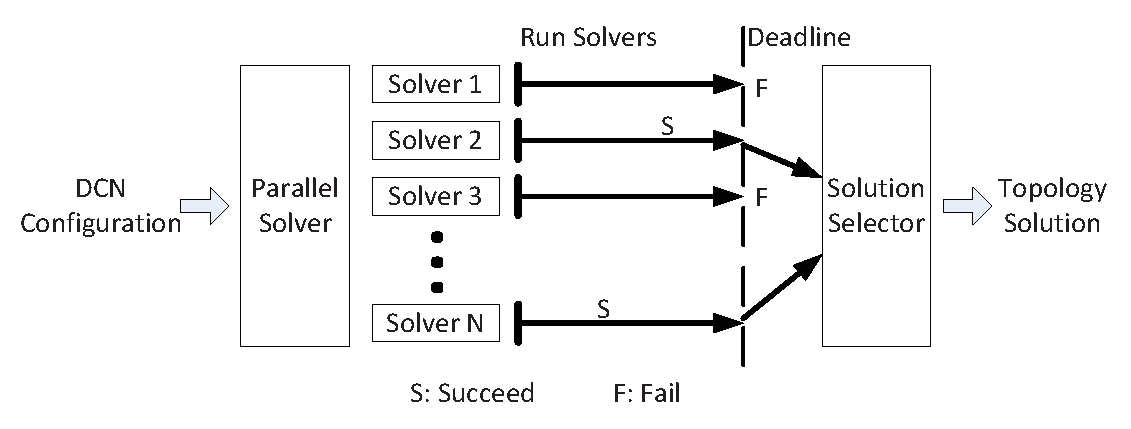
\includegraphics[scale=0.45]{parallel_solver}\\
\vspace{-1ex}
  \caption{Software architecture of the parallel solver.}\label{parallelsolver}
\end{figure}



\section{Changes to the Expansion Pipeline}\label{expansionplannersection}

The introduction of minimal rewiring requires several changes to the DCN expansion pipeline shown in Fig. \ref{expansionpipeline}.

Without minimal rewiring, it is fairly easy for an experienced network engineer to determine the number of stages required for an expansion; because almost all logical links need to be rewired,
we must use $C$ stages to maintain a residual capacity of $1-1/C$. 
With minimal rewiring, however, one cannot know the number of rewired links before running the solver; based on results in \S\ref{rewireratiosection}, the fraction could range from 0 to 30\%.

Therefore, we add an automated \textbf{expansion planner} step to the front of the pipeline in Fig. \ref{expansionpipeline}.  The planner first uses the minimal-rewiring solver to generate a post-expansion topology, then iteratively finds the lowest $C$, starting at $C=1$, which preserves the desired residual capacity threshold during the expansion (recall from \S\ref{PipelineSection} that this threshold is a function of forecasted demand, existing failures, and some headroom).
For each $C$, the planner divides the patch panels into $C$ groups, tentatively generates the $C$ intermediate topologies that would result from draining the affected links within a group, and evaluates those topologies against the threshold.  If capacity cannot be preserved for all intermediate topologies, the planner increments $C$ and tries again.  Once a suitable $C$ is found, the rest of the pipeline is safe to execute.

Without minimal rewiring, we simply drain all links for the patch panels covered by a stage.  Minimal rewiring allows us to preserve more capacity because we only have to drain a subset of the links, rather than an entire patch panel.   However, an operator can accidentally rewire the wrong link, or dislodge one inadvertently, a problem that does not occur when we drain entire panels.  Therefore, we built a link-status monitor that alerts the operator if an active (undrained) link is disconnected.  Since Clos networks by design tolerate some link failures, this allows the operator enough time to repair the problem without affecting users.\section{Experimental Results}

We have been successfully using this minimal-rewiring approach for our own DCNs since early 2017\footnote{Even though we have a formal proof that deaggregation always works, it does not guarantee optimality;
%~\cite{TechnicalReport}, 
our experience shows that our approach does work in practice.}. In order to demonstrate its benefits over a wide range of scales, we evaluated our approach using a set of synthetic DCN topologies (including some similar to our real DCNs), and show the effect of block aggregation on solver run-time and rewiring ratio.
We also show that our approach preserves most of the capacity of the original network during expansions, based on several workloads and under some failure scenarios.
 
\subsection{Synthesizing DCN Configurations}\label{dcn_configurations}

To evaluate our approach over a wide range of initial topologies, we synthesized thousands of configurations that were consistent with our past deployment experience.  In particular, since we must support heterogeneity among server blocks and spine blocks, we synthesized configurations using three types of server blocks and two types of spine block, in various combinations.  Every configuration includes exactly one “border block,” analogous to a server block but used for external connectivity.

%\begin{figure}
  %\centering
  %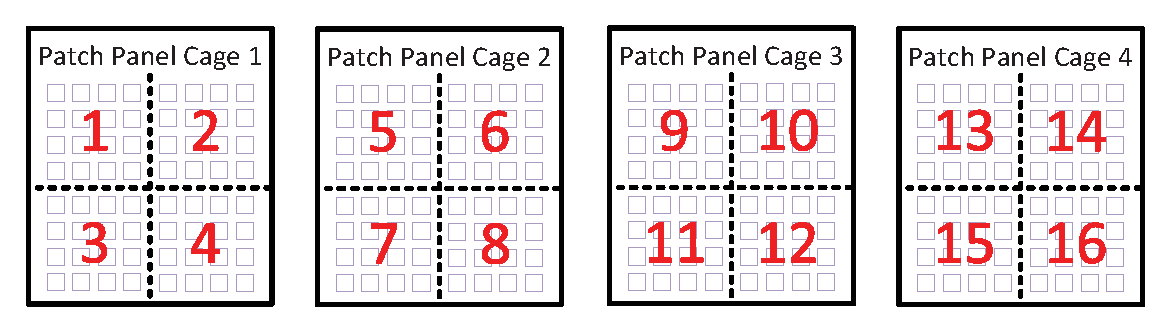
\includegraphics[scale=0.42]{cages}\\
  %\caption{Lay out of the 256 patch-panels.}\label{cages}
%\end{figure}

Our synthesized DCN configurations always have $256$ patch panels, located in $4$ sets, each with 64 patch panels. We use patch panels with 128 server-block-facing ports and 128 spine-block-facing ports, so the entire patch-panel layer supports up to 64 512-port server blocks.

Table \ref{blocktypes} lists the physical-topology parameters for the different block types. For example, a Type-1 server block has 512 up links, evenly distributed among all 256 patch panels. Type-2 \& Type-3 server blocks are ``light''  versions of the Type-1 server block, with fewer uplinks; they can be upgraded to Type-1 server blocks. Note that a Type-3 server block only connects to 128 patch panels. We divide the $256$ patch panels into two partitions, and connect the Type-3 server blocks to the two partitions by rotation. We also connect the Type-1 \& Type-2 spine blocks by rotation.

\begin{table}[ht]
\small
\centering
\caption{Server Block and Spine Block Types.}\label{blocktypes}
\begin{tabular}{| c | c | c | c |}
\hline
Block Type & Uplinks & Connected Patch Panels \\
\hline
Type-1 Server Block & 512 & 64 Per Set$\times$4 Sets\\
\hline
Type-2 Server Block & 256 & 64 Per Set$\times$4 Sets \\
\hline
Type-3 Server Block & 256 & 32 Per Set$\times$4 Sets \\
\hline
Border Block & 1024 & 64 Per Set$\times$4 Sets \\
\hline
Type-1 Spine Block & 128 & 64 Per Set$\times$1 Set \\
\hline
Type-2 Spine Block & 512 & 64 Per Set$\times$1 Set \\
\hline
\end{tabular}
\end{table}

We generate a total of 2250 initial configurations (pre-expansion ``reference topologies'' as defined in \S\ref{DefinitionsSection}) from all possible combinations of $\{3,6,...,30\}$ Type-1 server blocks, $\{2,4,...,20\}$ Type-2 server blocks, $\{3,6,...,30\}$ Type-3 server blocks, and $\{8, 16\}$ Type-1 spine blocks, with the remainder of the necessary spine-block ports as Type-2 spine blocks (the total number of server-block and spine-block ports must match).   We omit any configuration that would require more patch-panel ports than we have available.

\begin{comment}
\begin{algorithm}[ht]
\KwOut{A set of synthesized DCN configurations.}
    Initialize $\text{configuration\_set} = \{\}$.

    \tcc{Always set one border server block.}
    \text{border\_sb}=1\;

    \For {$\text{t1\_sb}\in \{3,6,...,30\}$} {
      \For {$\text{t2\_sb}\in \{2,4,...,20\}$} {
        \For {$\text{t3\_sb}\in \{3,6,...,30\}$} {
          $\text{total\_sb\_port}=\text{t1\_sb}\times 256+\text{t2\_sb}\times 512+\text{t3\_sb}\times 256+\text{border\_sb}\times 1024$\;
          \If {$\text{total\_sb\_port}>256\times 128$} {
            \tcc{$\text{total\_sb\_port}$ cannot exceed the total number of server-block facing Patch-Panel ports.}
            continue\;
          }
          \For {$\text{t1\_sp}\in\{8, 16\}$} {
            $\text{t2\_sp\_port}=\text{total\_sb\_port}-\text{t1\_sp}\times 128$\;

            $\text{t2\_sp}=\lceil\lceil\text{t2\_sp\_port}/512\rceil/4\rceil\times 4$\;

            $\text{config}=\text{GenerateConfig(t1\_sb, t2\_sb,}$ $\text{ t3\_sb, border\_sb, t1\_sp, t2\_sp)}$\;

            $\text{configuration\_set.Insert(config)}$\;
          }
        }
      }
    }
\caption{Generate DCN Configurations.}\label{generatepatterns}
\end{algorithm}
\end{comment}

These pre-expansion topologies can be generated using our minimal rewiring solver, by simply ignoring the objective function. We run all the configurations in parallel, and allocate 4 CPUs and 16G RAM for each configuration. With block aggregation enabled, all 2250 topologies can be computed within 10 seconds.

\subsection{Expansion Benchmarks}
As shown in Fig. \ref{dcnexpansion}, we support two types of DCN expansions. We construct two benchmarks for each of our 2250 reference topologies:

{\bf Benchmark Suite 1:} We upgrade two Type-2 server blocks in the reference topology to Type-1 server blocks.

{\bf Benchmark Suite 2:} We expand the reference topology by one Type-3 server block.

We end up with $2250 \times 2 = 4500$ total target topologies.  For each of these, we ran the minimal-rewiring solver with three aggregation strategies:
\begin{MYenum}
  \item No aggregation.
  \item Block aggregation, decomposing the spine-block and server-block layers using {\ifpaper ILP, \else ILP (\S\ref{minimalrewireilp}), \fi} while decomposing the patch-panel layer using MIN\_COST\_FLOW {\ifpaper (See technical report~\cite{TechnicalReport} for details) \else (\S\ref{deaggregationalgorithmsection}) \fi}.
  \item Block aggregation, decomposing all three layers using  MIN\_COST\_FLOW.
\end{MYenum}

\subsection{Solver scalability}\label{solverrunningtimesection}

\begin{figure}[ht]
  \centering
  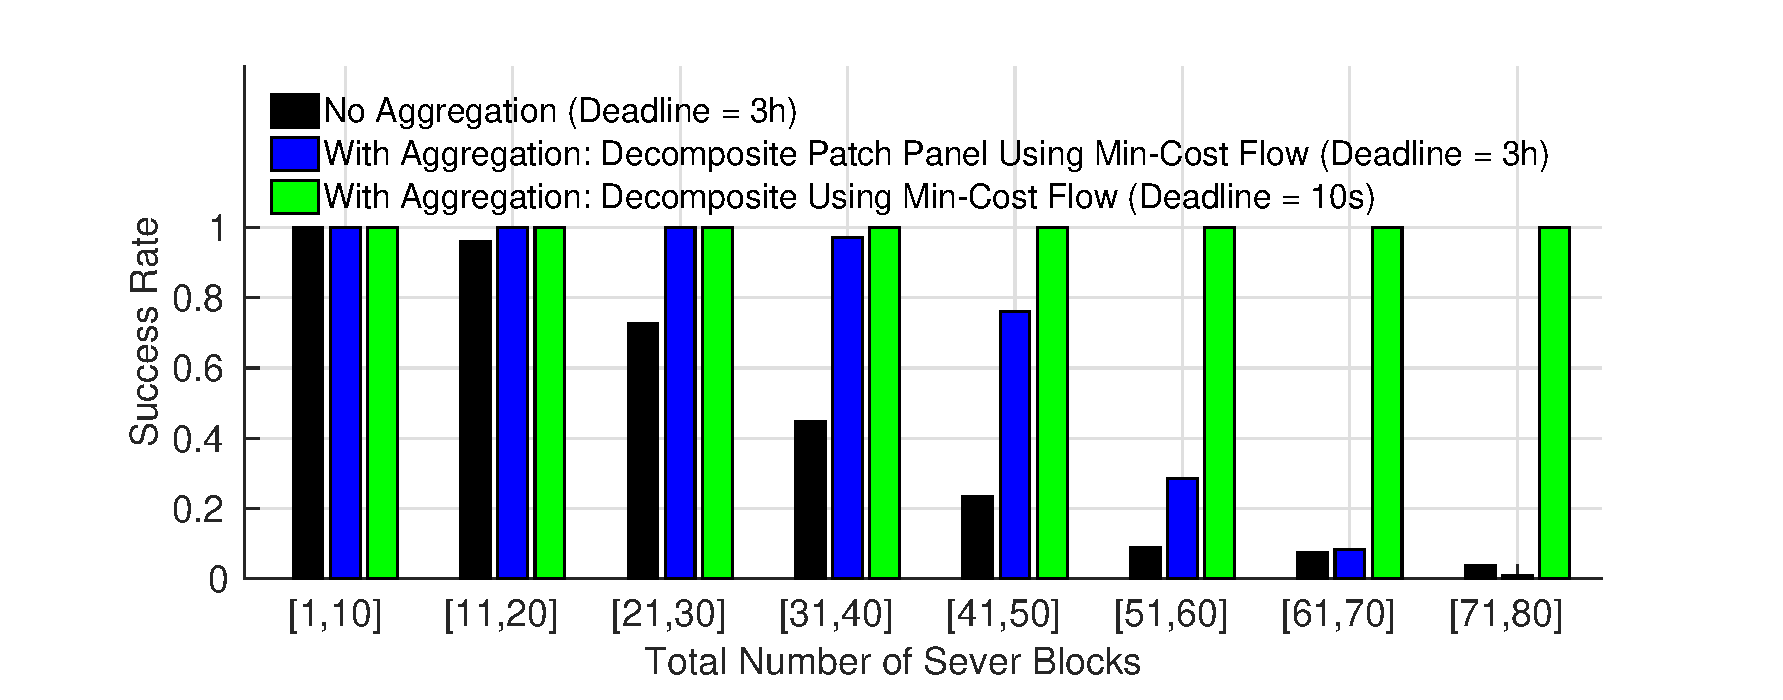
\includegraphics[scale=0.3]{incremental_size_success_rate}\\
\vspace{-1ex}
  \caption{Minimal-rewiring solver success rate.}\label{incremental_size_success_rate}
\end{figure}

Fig. \ref{incremental_size_success_rate} plots success rate for our minimal-rewiring solver with different aggregation strategies, grouped by the total number of server blocks; the bars show the fraction of topologies solved for each group.  With the third aggregation strategy, we can solve \emph{all} test cases within 10 seconds; this strategy only needs to solve one ILP for the aggregated problem, while using polynomial algorithms for all decompositions. The first strategy scales poorly, and can only solve 32\% of the test cases even if we increase the deadline to 3 hours; even for small DCNs (11--20 server blocks), it sometimes times out. The second strategy can solve 67\% of the test cases, but we start seeing timeouts for DCNs with 31--40 server blocks.  For all strategies, setting timeouts above 3 hours yields little improvement.

The differences between the second and third strategies shows that variable deaggregation using ILP could take significant run time. (If we also use ILP to deaggregate the patch-panel layer with the second strategy, only 3\% of the test cases can be solved.)  However, deaggregation via ILP is still useful, because as we discuss next, it can generate more-optimal rewiring solutions.

\subsection{Rewiring Ratio}\label{rewireratiosection}
\begin{figure}[ht]
  \centering
  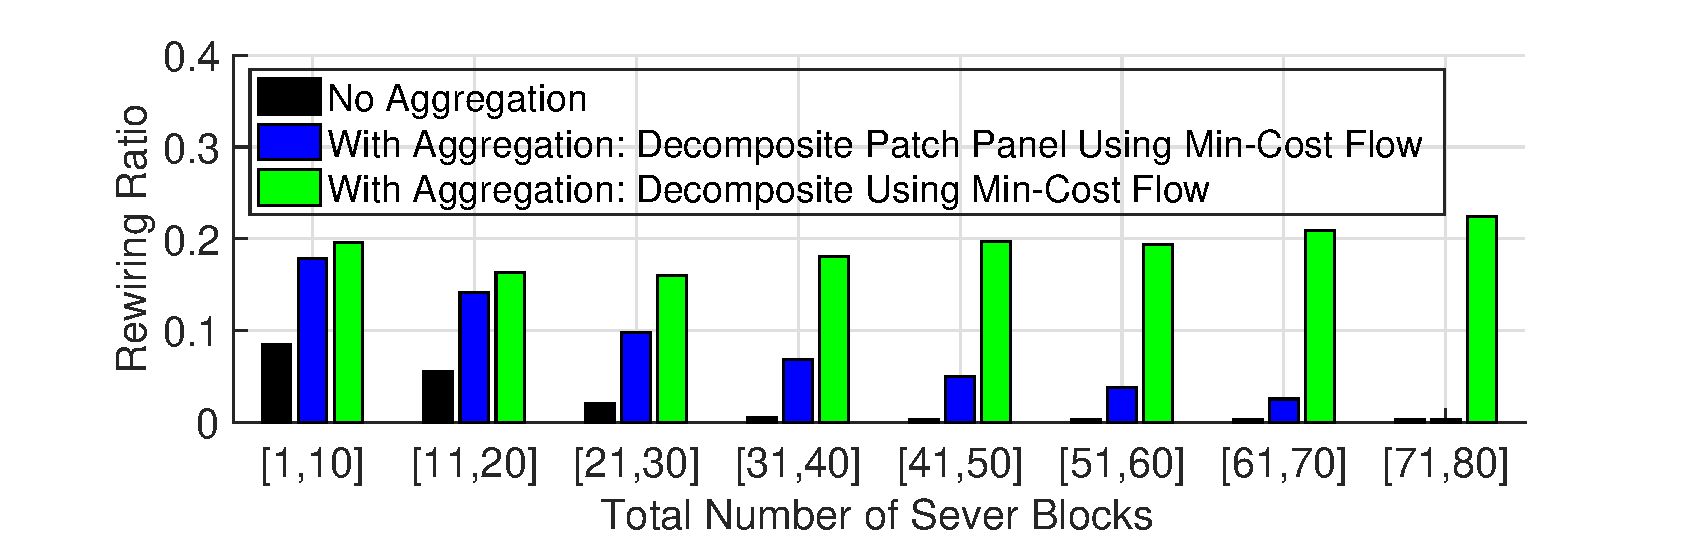
\includegraphics[scale=0.32]{incremental_rewire_ratio}\\  %50percentile
\vspace{-1ex}
  \caption{Mean rewiring ratio vs. aggregation strategy.}\label{incremental_rewire_ratio}
\end{figure}

For the same set of test cases, Fig. \ref{incremental_rewire_ratio} plots the rewiring ratios, again grouped by the number of server blocks; here, the bars show the mean value for each group. The third aggregation strategy, while it has the best run time, also leads to the highest (worst) rewiring ratio, often close to 20\%; this motivates our use of ILP for decomposition whenever we can tolerate the run time.

%Theoretically, we expect that the rewiring ratio for the solver without block aggregation would be the lowest. However, Fig. \ref{incremental_rewire_ratio} suggest that block aggregation with ILP-based deaggregation strategy can sometimes achieve even lower rewiring ratio. The only possibility we believe is that the ILP problem without block aggregation is too large that the true optimal solution cannot be generated. In fact, ILP problems are NP-hard. ILP problems with objective functions are usually solved using branch and bound. For large-scale ILP problems, it can be computationally impossible to exhaust all the possible branches, in which case the best possible feasible (but suboptimal) solution will be returned based on certain heuristics \cite{GurobiBasics}.

%Even though these rewriting ratios are much higher than those obtained using the other two aggregation strategies, it is still much better than not doing minimal rewiring. The main advantage of the min-cost-flow based variable-deaggregation strategy is that it is extremely fast and scalable. In case where a new topology needs to be computed immediately, this aggregation strategy can be used to compute a DCN topology with reasonably low rewiring ratio.

\subsection{Effectiveness of the parallel solver}
\label{ParallelRatioSection}

 \S\ref{parallelsolversection} described how we use a parallel solver to strike a balance between scalability and rewiring optimality.  For each of our benchmarks, we ran, in parallel, solvers with the three different aggregation strategies, with a 3-hour timeout. Because the third strategy works quickly for all instances, this parallel approach always succeeds. It also  achieves the best rewiring ratio available within a 3-hour budget.  Fig. \ref{parallelsolvercdf} plots the CDF of the parallel solver’s rewiring ratio. For about 82\% of the DCN configurations in the first benchmark suite, and about 93\% in the second suite, we get solutions with ratios under 20\%. (The first suite tends to yield a  higher ratio, because the total number of newly added server-block physical links in the first suite is twice that in the second suite.)

\begin{figure}
  \centering
  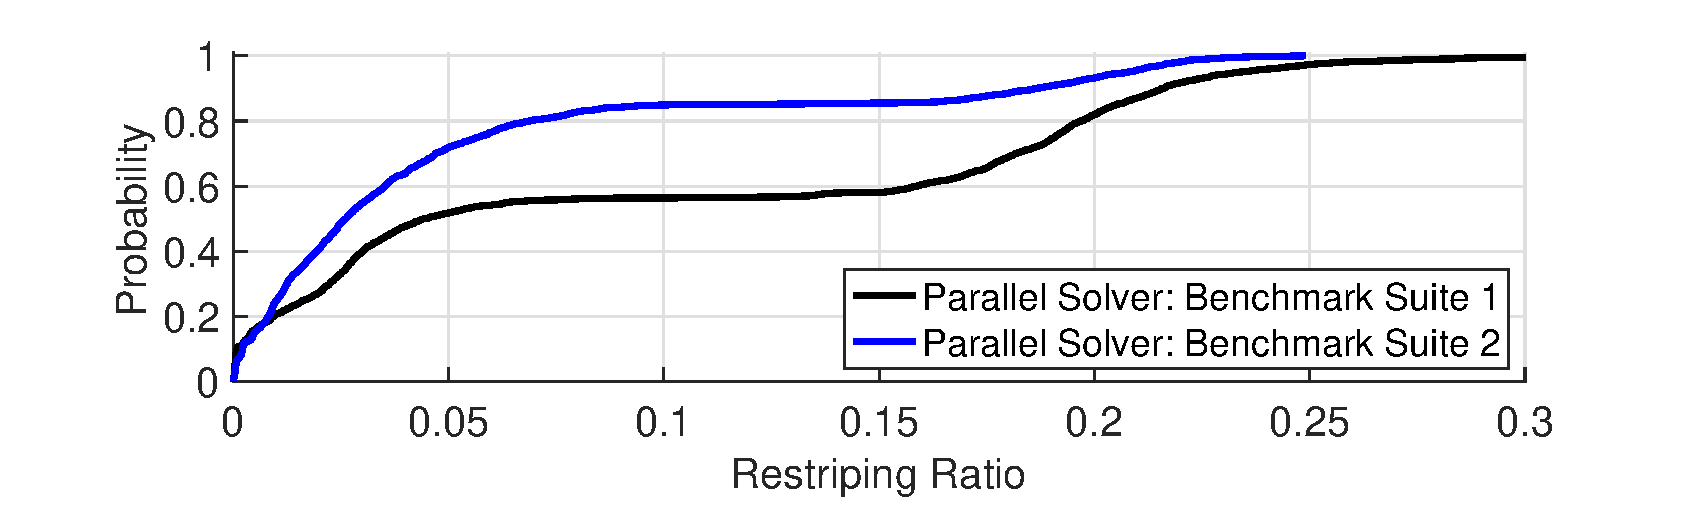
\includegraphics[scale=0.32]{parallel_rewire_ratio}\\
\vspace{-1ex}
  \caption{CDFs of rewiring ratios for the parallel solver.}\label{parallelsolvercdf}
\end{figure}

Note that the rewiring ratio for our prior approach was always 1.0 -- we always replaced all patch-panel jumpers. Fig. \ref{parallelsolvercdf}  shows that minimal rewiring saves us a lot of cost and time; the median rewiring ratio is about $22\times$ better for the first suite and about $38\times$ better for the second suite.

\subsection{Topology Capacity Analysis}\label{throughputanalysis}
In addition to solver scalability and rewiring optimality, we also must preserve sufficient capacity of the intermediate topologies during expansion.   This requires us to quantify ``capacity." While our DCNs experience a variety of traffic patterns, we specifically evaluate the maximum achievable capacity under one-to-all and one-to-one traffic, which we rigorously define as:

{\bf One-to-all capacity: $T_{\text{1-all}}$.} Assume that a source server block $E_n$ is sending traffic to all other server blocks, with its demand proportional to the ingress bandwidth of the destination blocks. We increase the traffic until some DCN links are fully utilized. Let $T_{\text{1-all}}^n$ be the ratio between the egress traffic under these assumptions and the best-case egress DCN bandwidth of the server block $E_n$. $T_{\text{1-all}}^n$ characterizes the one-to-all DCN capacity for server block $E_n$. We can then define $T_{\text{1-all}} = \min_{n=1}^N T_{\text{1-all}}^n$ as the one-to-all capacity of the entire DCN.

{\bf One-to-one capacity: $T_{\text{1-1}}$.} Assume that a server block $E_{n_1}$ is sending traffic to another server block $E_{n_2}$. We increase the traffic until some DCN links are fully utilized. Let $T_{\text{1-1}}^{n_1,n_2}$ be the ratio between the traffic sent and the minimum, over the two server blocks $E_{n_1}$ and $E_{n_2}$, of their ingress capacity. $T_{\text{1-1}}^{n_1,n_2}$ characterizes the one-to-one DCN capacity for the server blocks $E_{n_1}$ and $E_{n_2}$. We can then define $T_{\text{1-1}}=\min_{n_1\neq n_2} T_{\text{1-1}}^{n_1,n_2}$ as the one-to-one capacity of the entire DCN.

We evaluate $T_{\text{1-all}}$ and $T_{\text{1-1}}$ under two different scenarios:

{\bf Steady-state no-failures capacity:}
Recall that we imposed constraint (\ref{superspineblockconstraint}) when computing a topology, which ensures high capacity in the non-expansion steady state, without any failures. Ideally, if the $p_{n,m}$'s in (\ref{superspineblockconstraint}) were all integers, we would have $T_{\text{1-all}}=1$ and $T_{\text{1-1}}=1$. (Neither $T_{\text{1-all}}$ or $T_{\text{1-1}}$ can be larger than 1). Fig. \ref{throughput} plots CDFs of $T_{\text{1-all}}$ and $T_{\text{1-1}}$ based on the 4500 post-expansion topologies (benchmark suite 1 $+$ benchmark suite 2).  Note that both $T_{\text{1-all}}$ and $T_{\text{1-1}}$ are fairly close to 1.

{\bf Steady-state capacity under middle block failure:}
Recall that we imposed constraint (\ref{middlespineblockconstraint}), to ensure the highest possible capacity if one middle block fails. Ideally, for our typical case of 4 middle blocks, if the $q^t_{n,m}$'s in (\ref{middlespineblockconstraint}) were all integers, we would have $T_{\text{1-all}}=0.75$ and $T_{\text{1-1}}=0.75$, no matter which middle block fails. (Given one failure, neither $T_{\text{1-all}}$ or $T_{\text{1-1}}$ can be larger than $0.75$. Fig. \ref{throughput} also plots the CDFs of $T_{\text{1-all}}$ and $T_{\text{1-1}}$ under middle block failures. Note that both $T_{\text{1-all}}$ and $T_{\text{1-1}}$ are fairly close to 0.75.

%We analyze the throughput in both normal and failure scenarios. We use WCMP \cite{WCMP} as the routing policy\footnote{Due to the data center heterogeneity, ECMP \cite{ECMP} cannot achieve optimal throughput in our DCN.}, and compute throughput under both uniform traffic pattern and permutation traffic pattern.

\begin{figure}[ht]
  \centering
  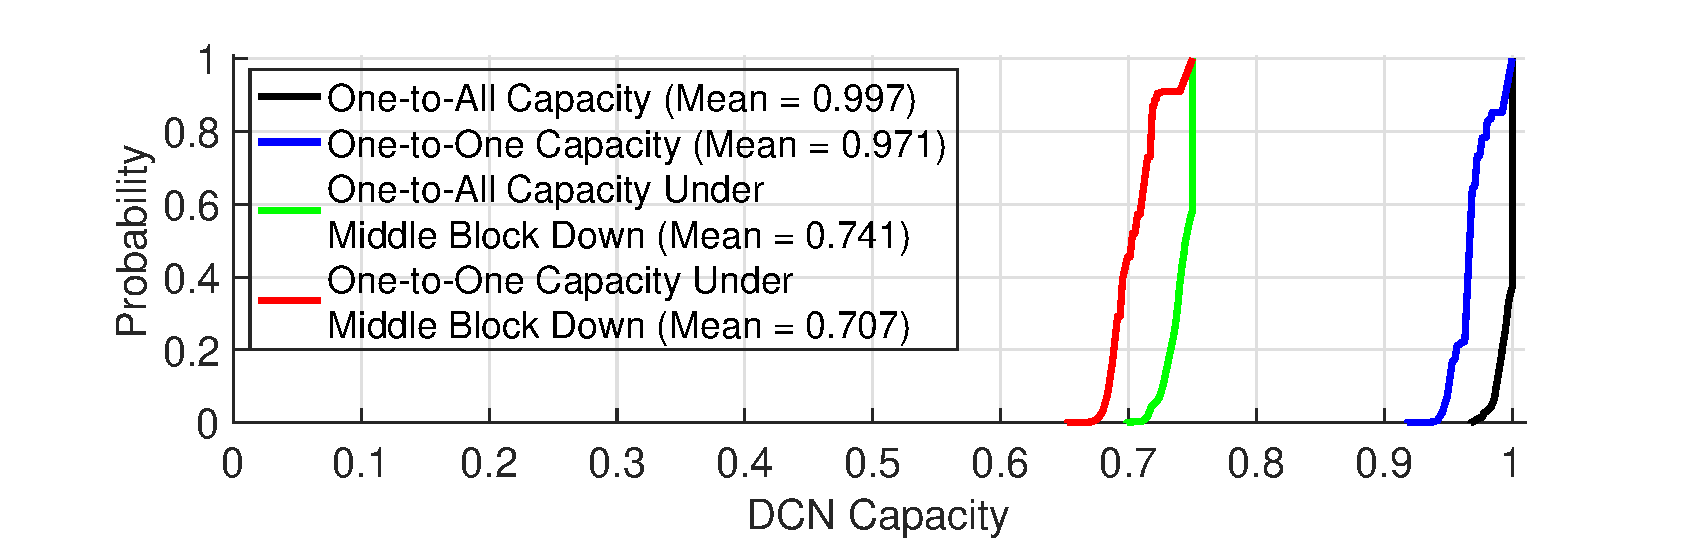
\includegraphics[scale=0.32]{throughput}\\
  \vspace{-1ex}
\caption{CDFs of One-to-All and One-to-One capacity.}\label{throughput}
\end{figure}

\subsubsection{Residual Capacity during Expansion}
During an expansion, we must disconnect some links, which reduces DCN capacity. We are interested in the residual capacity of the DCN in this state which clearly depends on the rewiring ratio. Fig. \ref{expansioncapacity}  shows scatter plots of  $T_{\text{1-all}}$ and $T_{\text{1-1}}$ for each (rewiring ratio, residual capacity) pair, based on the two benchmark suites.  This figure assumes we do all expansion in a single stage, even if the residual capacity is lower than we can accept in reality.

The residual capacity decreases approximately linearly with the rewiring ratio. Note that the residual capacity decreases faster than the rewiring ratio increase, because, the rewired DCN links might not be evenly distributed among different server blocks. As a result, some server blocks could suffer more capacity reduction than others.

\begin{figure}[ht]
  \centering
  \subfigure[$T_{\text{1-all}}$.]{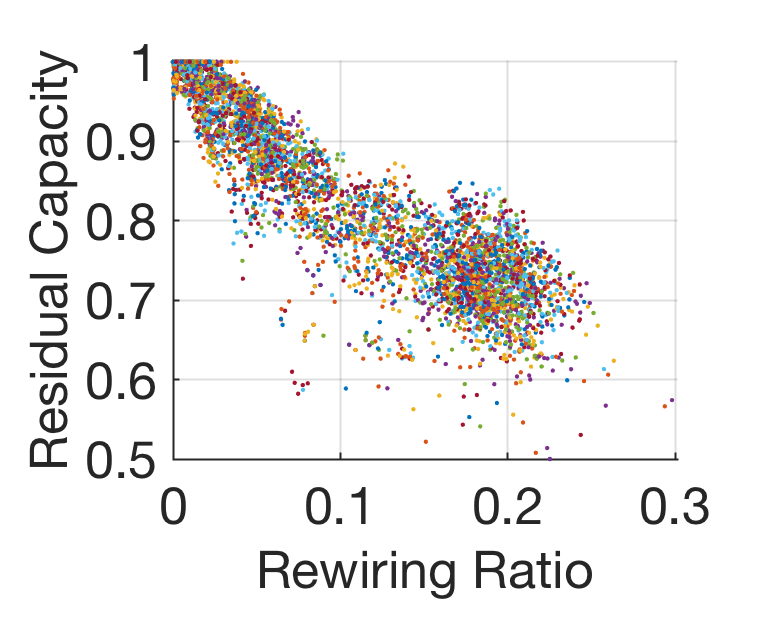
\includegraphics[scale=0.30]{uniform_capacity}}
  \subfigure[$T_{\text{1-1}}$.]{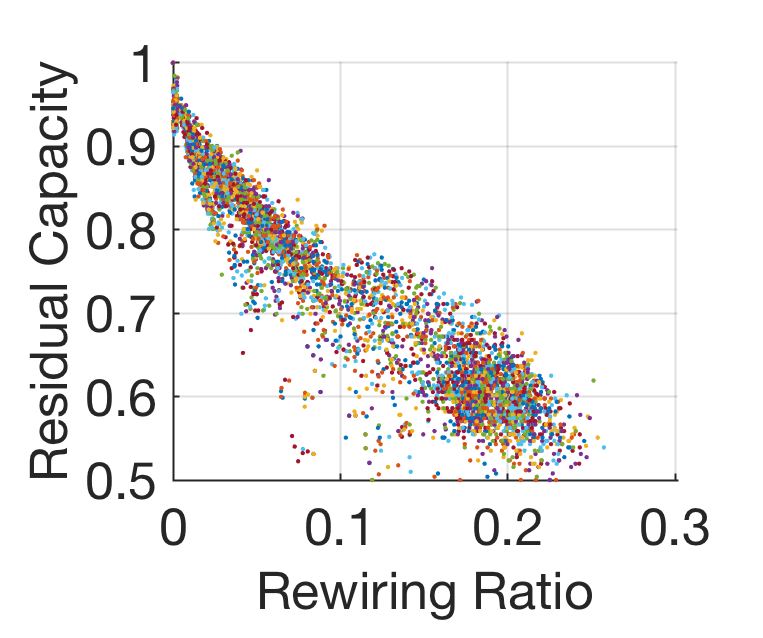
\includegraphics[scale=0.30]{permutation_capacity}}
\vspace{-1ex}
  \caption{Rewiring ratio \emph{vs.} residual capacity assuming a 1-stage expansion.}\label{expansioncapacity}
\end{figure}

\subsection{Number of expansion stages}
In practice, we might not be able to do an expansion in just one stage while preserving sufficient residual capacity. \S\ref{expansionplannersection} described an expansion planner that determines the number of stages required. We evaluated the number of stages saved by using minimal rewiring.

Prior to minimal rewiring, we typically did 4-stage expansions.  If the topologies were perfect, with 4 stages we could preserve a residual one-to-all capacity of 0.75, but in practice we cannot achieve perfect balance; we have found it feasible and sufficient to preserve a residual capacity of 0.7.

Table \ref{numstages} shows how many stages are needed to preserve a residual one-to-all capacity of 0.7, with minimal rewiring, for each of the 4500 benchmarks, based on solver strategy.  With strategies 1 and 2, many test cases require four stages, because the solvers time out before finding 1- or 2-stage expansions.  With strategy 3, almost all cases require at most 2 stages. The parallel solver finds 1- or 2-stage expansions for all test cases (because the few cases for which strategy 3 requires four stages are handled better by the other strategies), and usually does better than strategy 3 (because if the other strategies succeed within the deadline, they yield better rewiring ratios.)   Overall, the parallel solver needs an average of 1.29 stages, vs. 4 stages for our prior approach.


\begin{table}[ht]
\small
\centering
\caption{Number of expansion stages required.}\label{numstages}
\begin{tabular}{|c|c|c|c|}
\hline
Number of expansion stages: & 1 & 2 & 4  \\
\hline
\hline
Aggregation Strategy (1) & 1598 & 34 & 2868  \\
\hline
Aggregation Strategy (2) & 2668 & 416 & 1416  \\
\hline
Aggregation Strategy (3) & 1582 & 2914 & 4 \\
\hline
Parallel Solver & 3176 & 1324 & 0 \\
\hline
\end{tabular}
\\Cells show \# of test cases that need given \# of stages.
\end{table}

\subsubsection{Concrete example}\label{concrete_example}
A concrete (arbitrary, but realistic) example demonstrates the benefits of minimal rewiring.  Assume a pre-expansion DCN with 30 Type-1, 20 Type-2, 27 Type-3 server blocks, 1 border block, and 16 Type-1, 52 Type-2 spine blocks, which we expand by one Type-3 server block. Without minimal rewiring, we must rewire all the 28056 logical links, in four stages. With minimal rewiring, we need to rewire only 6063 of 28056 links (ratio $=0.216$), in two stages. Due to the scale of this example, only the third aggregation strategy succeeds. Table. \ref{casestudy} shows how this maintains mid-expansion capacity (in italics) higher than our prior approach (in bold), and completes in two stages rather than four.

\begin{table}[ht]
\small
\centering
\caption{Example: minimal rewiring vs. prior approach.}\label{casestudy}
\begin{tabular}{|c|c|c|c|c|c|c|}
\hline
 & \multicolumn{6}{c|}{Stage during expansion timeline} \\
\hline
 & Pre & 1 & 2 & 3 & 4 & Post  \\
\hline
\hline
Prior approach & 0.94 & \textbf{0.70} & \textbf{0.70} & \textbf{0.70} & \textbf{0.70} & 0.94  \\
\hline
Min. Rewiring & 0.94 & \textit{0.78} & \textit{0.78} & 0.94 & 0.94 & 0.94  \\
\hline
\end{tabular}
\\Cells show one-to-all capacity $T_{\text{1-all}}$ during expansion.
\end{table}

%\begin{figure}[ht]
  %\centering
  %\subfigure[$T_{\text{1-all}}$.]{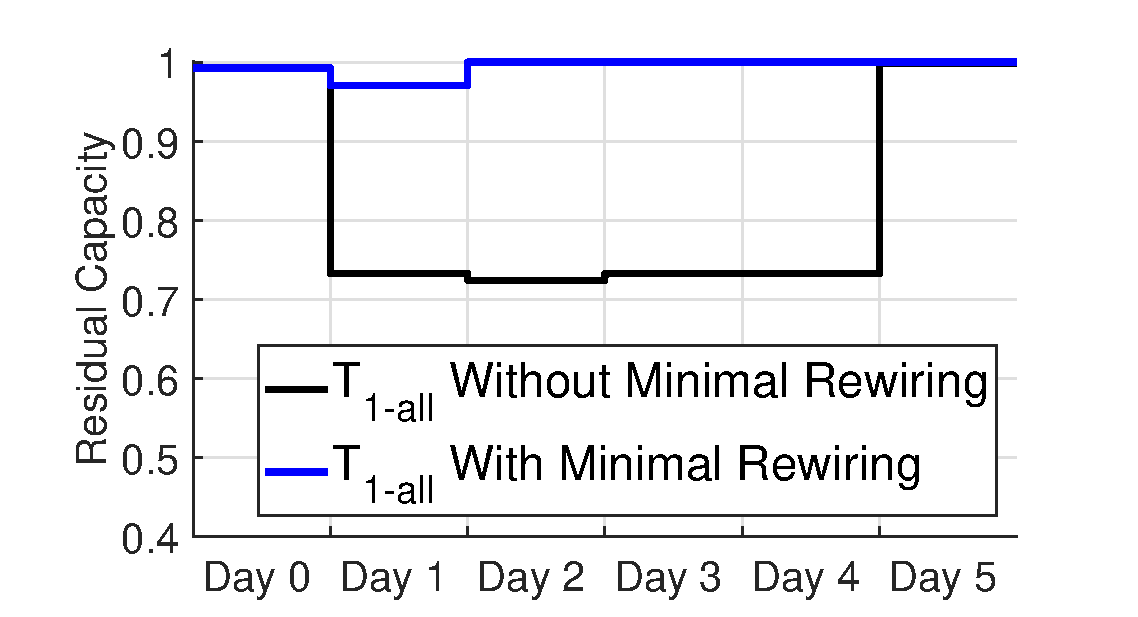
\includegraphics[scale=0.3]{uniform_case}}
  %\subfigure[$T_{\text{1-1}}$.]{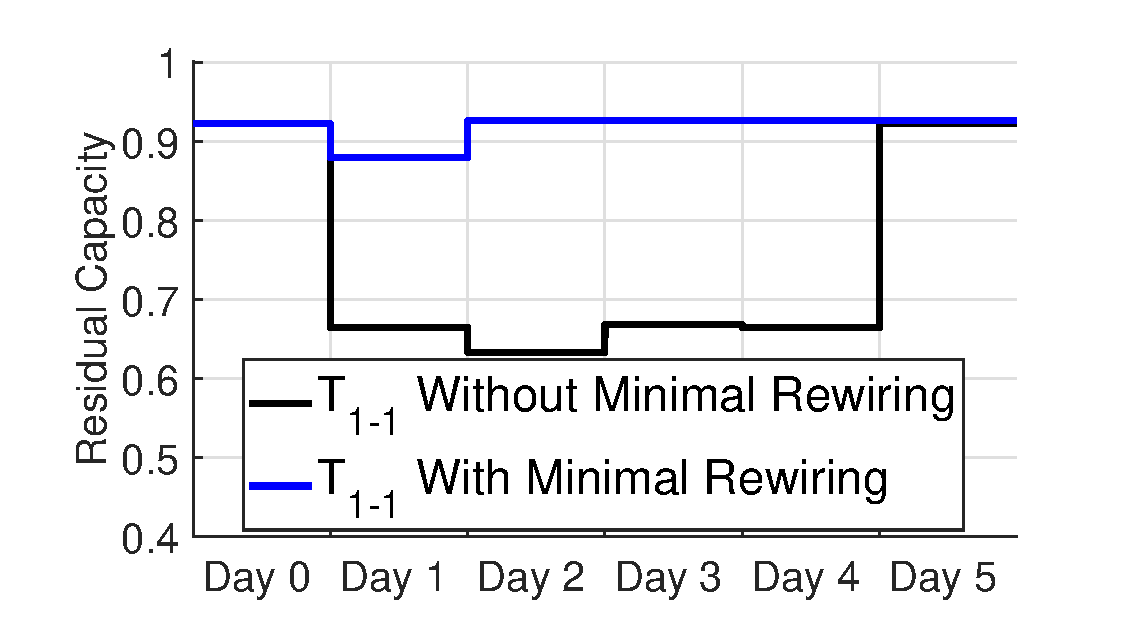
\includegraphics[scale=0.5]{permutation_case}}
  %\caption{Example: minimal rewiring vs. prior approach.}\label{casestudy}
%\emph{TODO(mogul@) can we mark ``end of expansion''?}
%\end{figure}


\section{Conclusion}
We have demonstrated that it is, in fact, feasible to do fine-grained expansions of heterogeneous Clos DCNs, at large scale, while preserving substantial residual capacity during an expansion, and with a significant reduction in the amount of rewiring (compared to prior approaches).  We described how we use a patch-panel layer to reduce the physical complexity of DCN expansions.  We then described an ILP formulation that allows us to minimize the amount of rewiring, a block-aggregation approach that allows scaling to large networks, and a parallel solver approach that yields the best tradeoff between elapsed time and rewiring ratio.   Our overall approach flexibly handles heterogenous switch blocks, and enforces ``balance’’ constraints that guarantee both high capacity and high failure resiliency. We evaluated our approach on a wide range of DCN configurations, and found on average that it allows us to do expansions in 1.29 stages, vs. 4 stages as previously required.

\section{Acknowledgements}
We thank Google colleagues for their insights and feedback, including Bob Felderman, David Wetherall, Keqiang He, Yadi Ma, Jad Hachem, Jayaram Mudigonda, and Parthasarathy Ranganathan. We also thank our shepherd Ankit Singla, and the NSDI reviewers.

\newpage
\bibliographystyle{acm}
\bibliography{zsz}

%\theendnotes


\clearpage
\appendix

\section{Matrix Decomposition}\label{matrixdecompositionsection}
We have proposed a block-aggregation technique to improve the scalability of our minimal-rewiring solver. By aggregating decision variables within different patch-panel groups, server-block groups and spine-block groups, the total number of decision variables is significantly reduced. However, the challenge here is that we must guarantee that the aggregated decision variables are also decomposable. Otherwise, no topology solution will be generated even if we can solve (\ref{minimalrewiringwithblockaggregation}).

In this section, we build an integer-matrix decomposition theory specifically for our block-aggregation technique. We will answer the following questions: 
\begin{enumerate}
  \item What are the requirements for matrix decomposition? 
  \item Under what circumstance will an integer matrix be decomposable?
  \item What algorithms can we use for integer-matrix decomposition?
\end{enumerate}

\subsection{A Sufficient Condition for Integer Matrix Decomposition}

We first introduce the following concepts:
\begin{defn}\label{powerset}
Given a set $\Omega$, the ``power set'' $\mathcal{P}(\Omega)$ of $\Omega$ is a set containing all the subsets of $\Omega$, including the empty set and $\Omega$ itself.
\end{defn}
\begin{defn}\label{goodset}
A subset $\mathcal{Q}\subset \mathcal{P}(\Omega)$ is called \emph{good}, if for any two sets $Q_1,Q_2\in\mathcal{Q}$, either (1) or (2) of the following conditions holds.

(1) $Q_1\cap Q_2=\emptyset$; (2) $Q_1\subset Q_2$ or $Q_2\subset Q_1$.
\end{defn}

A \emph{good} set has a very nice property, i.e., it can be represented by a set of trees. Specifically, we can construct a node for every element in the \emph{good} set, and create a directed link from $Q_1\in\mathcal{Q}$ to $Q_2\in\mathcal{Q}$ if and only if (1) $Q_2\subset Q_1$, and (2) there does not exist $Q_3\in\mathcal{Q}$ such that $Q_2\subset Q_3\subset Q_1$. An example is given in Fig. \ref{tree}. The concept of \emph{good} set is highly important. As readers will see shortly in Appendix \ref{decompositionsection}, constructing \emph{good} sets is actually the most critical step in variable deaggregation.
\begin{figure}[ht]
  \centering
  % Requires \usepackage{graphicx}
  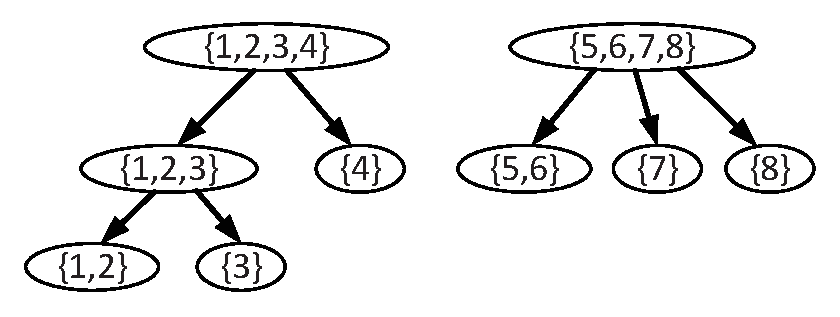
\includegraphics[scale=0.6]{tree}\\
  \caption{An example of \emph{good} set $\mathcal{Q}=\{\{1,2,3,4\},\{5,6,7,8\},\{1,2,3\},\{1,2\},\{3\},\{4\},\{5,6\},\{7\},$ $\{8\}\}$, and its tree representation.}\label{tree}
\end{figure}

Now, we are ready to introduce the following theorem on integer-matrix decomposition.

\begin{thm}\label{IMD}
Given an $I\times J$ non-negative integer matrix ${\bf x}=\{x_{i, j}\}$, and two sets $\mathcal{A}\subset\mathcal{P}(\{1,...,I\}), \mathcal{B}\subset\mathcal{P}(1,...,J)$, if both $\mathcal{A}$ and $\mathcal{B}$ are \emph{good}, then for any integer $H\geq 1$, there exist $H$ non-negative integer matrices ${\bf x^{(1)},...,x^{(H)}}$ satisfying
\begin{enumerate}
  \item ${\bf x}={\bf x^{(1)}+\cdots+x^{(H)}}$;
  \item for any $i=1,...,I, j=1,...,J$ and $h=1,2,...,H$,
   $$\left\lfloor \frac{x_{i,j}}{H}\right\rfloor\leq x^{(h)}_{i,j}\leq \left\lceil \frac{x_{i,j}}{H}\right\rceil;$$
  \item for any index set $A\in \mathcal{A}$ and any $h=1,2,...,H$,
   $$\left\lfloor \frac{\sum_{i\in A}\sum_{j=1}^J x_{i,j}}{H}\right\rfloor\leq\sum_{i\in A}\sum_{j=1}^J x^{(h)}_{i,j}\leq \left\lceil \frac{\sum_{i\in A}\sum_{j=1}^J x_{i,j}}{H}\right\rceil;$$
  \item for any index set $B\in \mathcal{B}$ and any $h=1,2,...,H$,
   $$\left\lfloor \frac{\sum_{i=1}^I\sum_{j\in B} x_{i,j}}{H}\right\rfloor\leq\sum_{i=1}^I\sum_{j\in B} x^{(h)}_{i,j}\leq \left\lceil \frac{\sum_{i=1}^I\sum_{j\in B} x_{i,j}}{H}\right\rceil.$$
\end{enumerate}
\end{thm}

The concept of \emph{good} set is critical for the correctness of Theorem \ref{IMD}. In practice, if either $\mathcal{A}$ or $\mathcal{B}$ is not \emph{good}, integer-matrix decomposition may fail. The following is a counter example.

\label{CounterExample} % keep the label with this text, so that it always refers to the right section
{\bf Counter Example:} Consider a $1\times 3$ matrix ${\bf x}=\{1, 1, 1\}$. Let $\mathcal{A}=\{\{1\}\}$, and $\mathcal{B}=\{\{1, 2\}, \{1, 3\}, \{2, 3\}\}$. Clearly, $\mathcal{B}$ is not \emph{good}. Further, if we let $H=2$, we can prove that no decomposition satisfies Condition (4) in Theorem \ref{IMD}. Specifically, Condition (4) requires that
\begin{eqnarray}
&&1 = \lfloor (1+1)/2 \rfloor \leq x^{(h)}_{1,1} + x^{(h)}_{1,2}\leq \lceil (1+1)/2 \rceil = 1,\nonumber\\
&&1 = \lfloor (1+1)/2 \rfloor \leq x^{(h)}_{1,1} + x^{(h)}_{1,3}\leq \lceil (1+1)/2 \rceil = 1,\nonumber\\
&&1 = \lfloor (1+1)/2 \rfloor \leq x^{(h)}_{1,2} + x^{(h)}_{1,3}\leq \lceil (1+1)/2 \rceil = 1.\nonumber
\end{eqnarray}
It is easy to verify that the above three inequalities do not have an integer solution.

Theorem \ref{IMD} is the key of variable deaggregation in our block-aggregation technique. Specifically, by aggregating decision variables, constraints are also aggregated. Thus, when we deaggregate the variables, we also need to make sure that the decomposed decision variables satisfy the original constraints. Theorem \ref{IMD} gives a sufficient condition under which a matrix can be ``evenly'' decomposed. As readers will see in Appendix \ref{decompositionsection}, this evenness makes sure that the decomposed variables satisfy the initial constraints before aggregation.

\subsection{Proof of Theorem \ref{IMD}}
We prove Theorem \ref{IMD} in this section. Specifically, we first introduce an algorithm that can compute an integer-matrix decomposition, and then prove that the decomposed integer matrices satisfy all the constraints in Theorem \ref{IMD}.

\subsubsection{Algorithm for Integer Matrix Decomposition}
The key is to transform the integer matrix decomposition problem into the following circulation problem.
\begin{defn}\label{circulation}
(Circulation Problem) Given a flow network with
\begin{itemize}
  \item $l(v,w)$, lower bound on flow from node $v$ to node $w$;
  \item $u(v,w)$, upper bound on flow from node $v$ to node $w$,
\end{itemize}
the goal of the circulation problem is to find a flow assignment $f(v,w)$ satisfying the following two constraints:
\begin{enumerate}
  \item $l(v,w)\leq f(v,w)\leq u(v,w)$;
  \item $\sum_u f(u,v) = \sum_w f(v,w)$ for any node $v$.
\end{enumerate}
\end{defn}

Given the \emph{good} sets $\mathcal{A}$ and $\mathcal{B}$ in Theorem \ref{IMD}, we can construct a circulation graph using the following steps (see Fig. \ref{flow} for an example):
\begin{enumerate}
  \item Create a directed bipartite graph. Note that ${\bf x}$ is an $I\times J$ matrix. We create $I$ nodes on the left hand side of the bipartite graph, and create $J$ nodes on the right hand side of the bipartite graph. We add a directed link from $i$ to $j$, and use $(i, j)$ to refer to this link.
  \item Construct a set of trees based on $\mathcal{A}$ on the left hand side of the bipartite graph. We add all the single-element sets to $\mathcal{A}$, and obtain $\mathcal{A}^{\prime}=\mathcal{A}\cup\{\{1\}, ...,\{I\}\}$. Since $\mathcal{A}$ is \emph{good}, it is easy to verify that $\mathcal{A}^{\prime}$ is also \emph{good}. Then, we construct a tree representation for $\mathcal{A}^{\prime}$ on the left hand side of the bipartite graph. We also introduce a dummy node, and create a directed link from this dummy node to all the root nodes in the tree representation. Note that each node $A\in\mathcal{A}^{\prime}$ on the left hand side has exactly one incoming link. Thus, with a little abuse of notation, we can use $A$ to refer to this link.
  \item Construct a tree representation, with all the links reversed, for $\mathcal{B}^{\prime}=\mathcal{B}\cup\{\{1\}, ...,\{J\}\}$ on the right hand side of the bipartite graph, and create a directed link from all the root nodes in the tree representation to the dummy node. Note that each node $B\in\mathcal{B}^{\prime}$ on the right hand side has exactly one outgoing link. Thus, we can use $B$ to refer to this link.
\end{enumerate}

\begin{figure}
  \centering
  % Requires \usepackage{graphicx}
  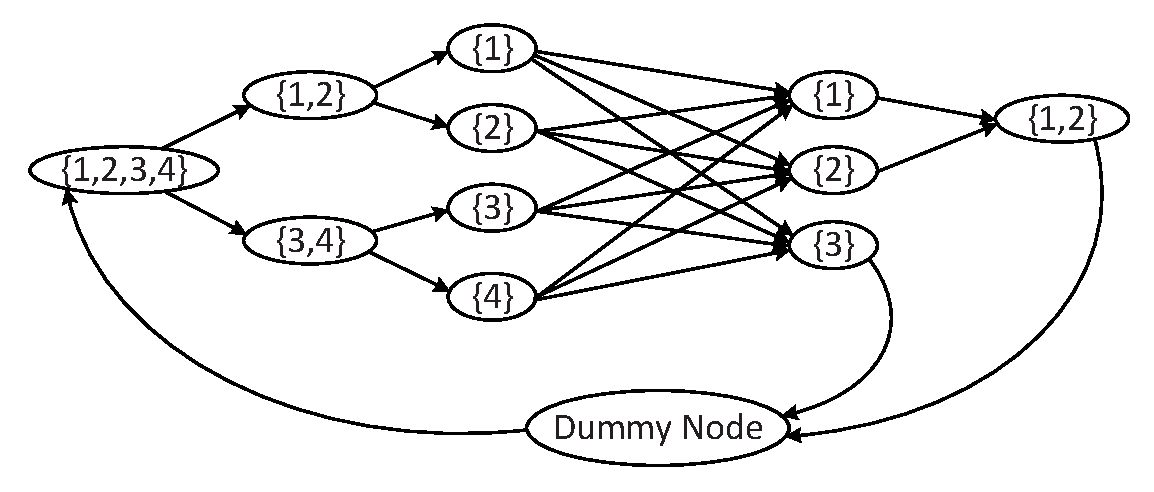
\includegraphics[scale=0.45]{flow}\\
  \caption{An example of circulation graph. Here, $I=4, J=3, \mathcal{A}=\{\{1,2,3,4\},\{1,2\},\{3,4\}\}, \mathcal{B}=\{\{1,2\},\{3\}\}$.}\label{flow}
\end{figure}

Given the above circulation graph, we can now introduce our integer-matrix decomposition algorithm (see Algorithm \ref{IMDAlgorithm}). The idea of Algorithm \ref{IMDAlgorithm} is to decompose the matrix {\bf x} iteratively. In each iteration, we first use the ``remaining part of $\bf x$'' to set bounds for the above circulation graph. We then compute an integer flow solution to the above circulation problem. Note that, circulation problems can be solved in polynomial time by the Goldberg-Tarjan algorithm \cite{PreFlow}. Finally, we map the integer flow solution to a decomposed integer matrix.

\begin{algorithm}[ht]
\KwIn{${\bf x}=\{x_{i, j}\}$, and two good sets $\mathcal{A}$ and $\mathcal{B}$.}
\KwOut{${\bf x^{(1)},...,x^{(H)}}$}
  \tcc{Use $\bf \hat{x}^{(h)}$ to track the remaining part of $\bf x$.}
  Let $\bf \hat{x}^{(H)} = \bf x$.

  \For{$h = H;\ h \geq 1;\ h--$}{
    \tcc{Assign bounds to the circulation graph.}
    \For {any bipartite graph link $(i,j)$} {
      Set its bound as $\left[\left\lfloor \hat{x}^{(h)}_{i,j}/{h}\right\rfloor, \left\lceil \hat{x}^{(h)}_{i,j}/{h}\right\rceil\right]$\;
    }
    \tcc{Note that there are no bounds assigned to the links in $\mathcal{A}^{\prime}\setminus\mathcal{A}$ and $\mathcal{B}^{\prime}\setminus\mathcal{B}$.}
    \For {any link $A$ in $\mathcal{A}$} {
      Set its bound as $[\lfloor (\sum_{i\in A}\sum_{j=1}^J \hat{x}^{(h)}_{i,j})/{h}\rfloor, \lceil (\sum_{i\in A}\sum_{j=1}^J \hat{x}^{(h)}_{i,j})/{h}\rceil]$\;
    }
    \For {any any link $B$ in $\mathcal{B}$} {
      Set its bound as $[\lfloor (\sum_{i=1}^I\sum_{j\in B} \hat{x}^{(h)}_{i,j})/{h}\rfloor, \lceil (\sum_{i=1}^I\sum_{j\in B} \hat{x}^{(h)}_{i,j})/{h}\rceil]$\;
    }

    Compute an integer solution to the above circulation problem\;

    \For {any bipartite graph link $(i,j)$} {
      Let ${\bf x^{(h)}_{i,j}} = \text{ Amount of flow on the link } (i,j)$\;
    }

    Let ${\bf \hat{x}^{(h-1)}} = {\bf \hat{x}^{(h)}} -{\bf x^{(h)}}$\;
  }
\caption{Integer-Matrix Decomposition Algorithm.}\label{IMDAlgorithm}
\end{algorithm}

Note that, there are two caveats in Algorithm  \ref{IMDAlgorithm}. First, how can we guarantee that the circulation graph generated above always has a solution? Second, why does the integer matrix obtained in each iteration satisfy all the constraints in Theorem \ref{IMD}. Next, we will prove them one by one.

\subsubsection{Correctness of Algorithm \ref{IMDAlgorithm}}\label{correctnessproofsection}
Based on our earlier discussion, the proof consists of two steps.

{\bf Step 1: The circulation problem constructed in Algorithm \ref{IMDAlgorithm} always has an integer solution.}

The proof of Step 1 requires the following lemma.
\begin{lem}\label{integralflowtheorem}
(Integral Flow Theorem) Given a feasible circulation problem, if $l(v,w)$'s and $u(v,w)$'s are all integers, then there exists a feasible flow assignment such that all flows are integers.
\end{lem}
In fact, for feasible circulation problems with integer bounds, most max-flow algorithms, e.g., Edmonds-Karp algorithm \cite{FlowAlgorithm} and Goldberg-Tarjan algorithm \cite{PreFlow}, are guaranteed to generate integer solutions.

According to Lemma \ref{integralflowtheorem}, we only need to prove that the circulation problem constructed in Algorithm \ref{IMDAlgorithm} is feasible. Specifically, we can assign fractional network flows as follows:
\begin{itemize}
  \item for the link $(i,j)$, assign $\hat{x}^{(h)}_{i,j}/{h}$ amount of flow;
  \item for the link $A\in\mathcal{A}^{\prime}$, assign $(\sum_{i\in A}\sum_{j=1}^J \hat{x}^{(h)}_{i,j})/{h}$ amount of flow;
  \item for the link $B\in\mathcal{B}^{\prime}$, assign $(\sum_{i=1}^I\sum_{j\in B} \hat{x}^{(h)}_{i,j})/{h}$ amount of flow.
\end{itemize}
It is easy to verify that the above fractional flow assignment satisfies the two constraints in the Definition \ref{circulation}. Thus, the circulation problem in Algorithm \ref{IMDAlgorithm} is feasible. Note that all the bounds of this circulation problem are all integers. If we use Edmonds-Karp algorithm or Goldberg-Tarjan algorithm to compute a flow assignment, there is a guaranteed integer solution.

{\bf Step 2: ${\bf x^{(1)},...,x^{(H)}}$ satisfy Conditions (1)-(4) of Theorem \ref{IMD}.}

The proof of Step 2 requires the following lemma.
\begin{lem}\label{floorceilinequality}
Given positive integers $y, z, h$ satisfying $\lfloor y/(h+1) \rfloor\leq z \leq \lceil y/(h+1)\rceil$, the following inequality holds $$\lfloor y/(h+1) \rfloor\leq \lfloor (y-z)/h \rfloor\leq \lceil (y-z)/h\rceil \leq \lceil y/(h+1)\rceil.$$
\end{lem}

Since $\bf x^{(h)}$ is an integer solution to the circulation problem constructed in Algorithm \ref{IMDAlgorithm}, $\bf x^{(h)}$ must satisfy the following constraints:
\begin{description}
  \item[$2^{\prime})$] for any $i=1,...,I, j=1,...,J$ and $h=1,2,...,H$,
   $$\left\lfloor \frac{\hat{x}^{(h)}_{i,j}}{h}\right\rfloor\leq x^{(h)}_{i,j}\leq \left\lceil \frac{\hat{x}^{(h)}_{i,j}}{h}\right\rceil;$$
  \item[$3^{\prime})$] for any index set $A\in \mathcal{A}$ and any $h=1,2,...,H$,
   $$\left\lfloor \frac{\sum_{i\in A}\sum_{j=1}^J \hat{x}^{(h)}_{i,j}}{h}\right\rfloor\leq\sum_{i\in A}\sum_{j=1}^J x^{(h)}_{i,j}\leq \left\lceil \frac{\sum_{i\in A}\sum_{j=1}^J \hat{x}^{(h)}_{i,j}}{h}\right\rceil;$$
  \item[$4^{\prime})$] for any index set $B\in \mathcal{B}$ and any $h=1,2,...,H$,
   $$\left\lfloor \frac{\sum_{i=1}^I\sum_{j\in B} \hat{x}^{(h)}_{i,j}}{h}\right\rfloor\leq\sum_{i=1}^I\sum_{j\in B} x^{(h)}_{i,j}\leq \left\lceil \frac{\sum_{i=1}^I\sum_{j\in B} \hat{x}^{(h)}_{i,j}}{h}\right\rceil.$$
\end{description}

Let $h=1$ in ($2^{\prime}$). We obtain ${\bf x}^{(1)} = {\bf \hat{x}}^{(1)}$. Thus,
$${\bf x}= {\bf \hat{x}}^{(1)} + {\bf x}^{(2)} + \cdots + {\bf x}^{(H)} = {\bf x^{(1)}+\cdots+x^{(H)}}.$$

It remains to prove that ($2^{\prime}$)($3^{\prime}$)($4^{\prime}$) imply the constraints (2)(3)(4) in Theorem \ref{IMD}. The constraints (2)(3)(4) can be proved using similar techniques. Here, we take (2) as an example.

Note that $\hat{x}^{(h)}_{i,j} = \hat{x}^{(h+1)}_{i,j} - x^{(h+1)}_{i,j}$ and $\left\lfloor \hat{x}^{(h+1)}_{i,j}/(h+1)\right\rfloor\leq x^{(h+1)}_{i,j}\leq \left\lfloor \frac{\hat{x}^{(h)}_{i,j}}{h}\right\rfloor\leq \left\lceil \hat{x}^{(h+1)}_{i,j}/(h+1)\right\rceil$. According to Lemma \ref{floorceilinequality}, we immediately have
$$\left\lfloor \frac{\hat{x}^{(h+1)}_{i,j}}{h+1}\right\rfloor \leq \left\lfloor \frac{\hat{x}^{(h)}_{i,j}}{h}\right\rfloor\leq x^{(h)}_{i,j}\leq \left\lceil \frac{\hat{x}^{(h)}_{i,j}}{h}\right\rceil \leq \left\lceil \frac{\hat{x}^{(h+1)}_{i,j}}{h+1}\right\rceil.$$
Repeat the above analysis, we then have
$$\left\lfloor \frac{x_{i,j}}{H}\right\rfloor = \left\lfloor \frac{\hat{x}^{(H)}_{i,j}}{H}\right\rfloor\leq x^{(h)}_{i,j}\leq \left\lceil \frac{\hat{x}^{(H)}_{i,j}}{H}\right\rceil = \left\lceil \frac{x_{i,j}}{H}\right\rceil.$$

\subsection{``Minimal Rewiring'' for Integer Matrix Decomposition}
We have proved the integer matrix decomposition Theorem \ref{IMD}. As a byproduct, we also obtain an algorithm that can accomplish the decomposition in polynomial time (see Algorithm \ref{IMDAlgorithm}). As readers will see in Appendix \ref{decompositionsection}, these results guarantee that the solutions of (\ref{minimalrewiringwithblockaggregation}) are always decomposable. However, none of these results can be used for variable deaggregation due to the objective function in (\ref{mrstep2}). In this section, we study how to do integer-matrix decomposition when we have an minimal-rewiring objective function of the following form:
\begin{equation}\label{fakeminimalrewiring}
\min\sum_{h=1}^H\sum_{i=1}^I\sum_{j=1}^J(b_{i,j}^{(h)} - x_{i,j}^{(h)})^+,
\end{equation}
where $\bf b^{(1)},...,\bf b^{(H)}$ are $I\times J$ reference matrices for decomposition.

We introduce two approaches for the minimal-rewiring integer-matrix decomposition problem in the following.

\subsubsection{ILP based Approach}\label{minimalrewireilp}
The first one is based on integer linear programming. Specifically, we note that $(b_{i,j}^{(h)} - x_{i,j}^{(h)})^+$ can be positive only if $b_{i,j}^{(h)} > \lfloor x_{i,j}/{H}\rfloor$ because $x_{i,j}^{(h)}$ needs to satisfy the second constraint in Theorem \ref{IMD}. Hence, the minimal-rewiring integer-matrix decomposition problem can be formulated as the following ILP problem:
\begin{eqnarray}\label{fakeminimalrewiringformulation}
&\min_{{\bf x^{(h)}}}&\sum_{b_{i,j}^{(h)} > \lfloor x_{i,j}/{H}\rfloor}(b_{i,j}^{(h)} - x_{i,j}^{(h)}),\\
&\text{subject to}&\text{constraints (1)-(4) in Theorem \ref{IMD}.}\nonumber
\end{eqnarray}

\subsubsection{Min-Cost-Flow based Approach}\label{deaggregationalgorithmsection}
The second approach is based on the min-cost flow problem. Similar to the Circulation problem in Definition \ref{circulation}, we introduce the following min-cost circulation problem.

\begin{algorithm}[!htbp]
\KwIn{${\bf x}=\{x_{i, j}\}$, two good sets $\mathcal{A}$ and $\mathcal{B}$, and $H$ base matrices ${\bf b^{(1)},...,b^{(H)}}$.}
\KwOut{${\bf x^{(1)},...,x^{(H)}}$}
  \tcc{Use $\bf \hat{x}^{(h)}$ to track the remaining part of $\bf x$.}
  Let $\bf \hat{x}^{(H)} = \bf x$.

  \For{$h = H;\ h \geq 1;\ h--$}{
    Initialize the cost of all the links as 0.

    \tcc{Assign bounds to the circulation graph.}
    \For {any bipartite graph link $(i,j)$} {
      Set its bound as $\left[\left\lfloor \hat{x}^{(h)}_{i,j}/{h}\right\rfloor, \left\lceil \hat{x}^{(h)}_{i,j}/{h}\right\rceil\right]$\;

      \If {$b^{(h)}_{i,j} > \lfloor x_{i,j}/{H}\rfloor$} {
        Set the cost of the link $(i,j)$ as $-1$\;
      }
    }
    \tcc{Note that there are no bounds assigned to the links in $\mathcal{A}^{\prime}\setminus\mathcal{A}$ and $\mathcal{B}^{\prime}\setminus\mathcal{B}$.}
    \For {any link $A$ in $\mathcal{A}$} {
      Set its bound as $[\lfloor (\sum_{i\in A}\sum_{j=1}^J \hat{x}^{(h)}_{i,j})/{h}\rfloor, \lceil (\sum_{i\in A}\sum_{j=1}^J \hat{x}^{(h)}_{i,j})/{h}\rceil]$\;
    }
    \For {any any link $B$ in $\mathcal{B}$} {
      Set its bound as $[\lfloor (\sum_{i=1}^I\sum_{j\in B} \hat{x}^{(h)}_{i,j})/{h}\rfloor, \lceil (\sum_{i=1}^I\sum_{j\in B} \hat{x}^{(h)}_{i,j})/{h}\rceil]$\;
    }

    Compute an integer solution to the above min-cost circulation problem\;

    \For {any bipartite graph link $(i,j)$} {
      Let ${\bf x^{(h)}_{i,j}} = \text{ Amount of flow on the link } (i,j)$\;
    }

    Let ${\bf \hat{x}^{(h-1)}} = {\bf \hat{x}^{(h)}} -{\bf x^{(h)}}$\;
  }
\caption{A Min-Cost Flow based Integer-Matrix Decomposition Algorithm.}\label{MrIMDAlgorithm}
\end{algorithm}

\begin{defn}\label{mincostcirculation}
(Min-Cost Circulation Problem) Given a flow network with
\begin{itemize}
  \item $l(v,w)$, lower bound on flow from node $v$ to node $w$;
  \item $u(v,w)$, upper bound on flow from node $v$ to node $w$;
  \item $c(v,w)$, cost of a unit of flow on $(v,w)$,
\end{itemize}
the goal of the min-cost circulation problem is to find a flow assignment $f(v,w)$ that minimizes
$$\sum_{(v,w)}c(v,w)\cdot f(v,w),$$
while satisfying the following two constraints:
\begin{enumerate}
  \item $l(v,w)\leq f(v,w)\leq u(v,w)$;
  \item $\sum_u f(u,v) = \sum_w f(v,w)$ for any node $v$.
\end{enumerate}
\end{defn}

Similar to the circulation problem, the min-cost circulation problem can be also solved in polynomial time using the Goldberg-Tarjan min-Cost flow algorithm \cite{MinCostFlowImplementation}.

With the above min-cost circulation problem, we can slightly modify Algorithm \ref{IMDAlgorithm} to obtain an algorithm for the minimal-rewiring integer-matrix decomposition problem. Specifically, we introduce a weight to all the bipartite graph links $(i, j)$ (see lines 6-8 in Algorithm \ref{MrIMDAlgorithm}), and then use the min-Cost flow algorithm to compute a flow solution (see line 16 in Algorithm \ref{MrIMDAlgorithm}). Then, at each iteration, we obtain a new decomposed matrix that minimizes the total rewiring, i.e., $\sum_{i=1}^I\sum_{j=1}^J(b_{i,j}^{(h)} - x_{i,j}^{(h)})^+$.

Compared to the ILP-based approach, the min-cost-flow based approach has significantly lower complexity. However, the solution of the min-cost-flow based approach can be suboptimal. Algorithm \ref{MrIMDAlgorithm} is essentially a greedy algorithm that optimizes (\ref{fakeminimalrewiring}) in multiple steps. In practice, both approaches are useful. When the ILP-based approach can compute a solution within tolerable time, use the ILP-based approach. When users care more about run-time complexity, use the min-cost-flow based approach.

\section{Variable Deaggregation}\label{decompositionsection}
With the newly-developed integer-matrix decomposition theory (see Appendix \ref{matrixdecompositionsection}), we are now ready to decompose the aggregated decision variables $d^*_{k_g}(E_{n_g}^t, S_{m_g})$ in this section. Instead of solving (\ref{mrstep2}) directly, we decompose $d^*_{k_g}(E_{n_g}^t, S_{m_g})$ in three steps: patch-panel decomposition, server block decomposition, and spine block decomposition. The general idea is to apply the integer matrix decomposition theory in each step.  Patch-panel decomposition is easier, and thus will be discussed first. Server block decomposition and spine block decomposition are more involved, and thus will be discussed later. We note that server block decomposition and spine block decomposition are very similar. So we will only discuss server block decomposition in the following.

\subsection{Patch-Panel Decomposition}
In this section, we decompose $d^*_{k_g}(E_{n_g}^t, S_{m_g})$ to $d^*_{k}(E_{n_g}^t, S_{m_g})$. $d^*_{k}(E_{n_g}^t, S_{m_g})$ can be also viewed as an aggregated variable of $d^*_{k}(E_n^t, S_m)$. Thus, $d^*_{k}(E_{n_g}^t, S_{m_g})$ must satisfy the following constraints:
\begin{equation}\label{blockaggregateblockdecisionvariables1}
0\leq d^*_{k}(E_{n_g}^t, S_{m_g})\leq |n_g||m_g|\min\{G_k(E_n^t), G_k(S_m)\}.
\end{equation}
\begin{equation}\label{blockaggregatesuperblockconnect1}
\sum_{m_g=1}^{M_g}d^*_{k}(E_{n_g}^t, S_{m_g}) = |n_g|G_k(E_n^t).
\end{equation}
\begin{equation}\label{blockaggregatespineblockconnect1}
\sum_{n_g=1}^{N_g}\sum_{t=1}^4d^*_{k}(E_{n_g}^t, S_{m_g}) \leq |m_g|G_k(S_m).
\end{equation}
\begin{equation}\label{blockaggregatesuperspineblockconstraint1}
|n_g||m_g|\lfloor p_{n,m}\rfloor\leq \sum_{k=1}^{K}\sum_{t=1}^4 d^*_{k}(E_{n_g}^t, S_{m_g})\leq |n_g||m_g|\lceil p_{n,m}\rceil.
\end{equation}
\begin{equation}\label{blockaggregatemiddlespineblockconstraint1}
|n_g||m_g|\lfloor q^t_{n,m}\rfloor\leq \sum_{k=1}^{K}d^*_{k}(E_{n_g}^t, S_{m_g})\leq |n_g||m_g|\lceil q^t_{n,m}\rceil.
\end{equation}

Note that $d^*_{k_g}(E_{n_g}^t, S_{m_g})$ satisfies (\ref{blockaggregatesuperspineblockconstraint}) and (\ref{blockaggregatemiddlespineblockconstraint}), then (\ref{blockaggregatesuperspineblockconstraint1}) and (\ref{blockaggregatemiddlespineblockconstraint1}) hold as long as $d^*_{k_g}(E_{n_g}^t, S_{m_g})=\sum_{k\in k_g}d^*_{k}(E_{n_g}^t, S_{m_g})$. Then, the patch-panel decomposition problem can be precisely formulated as follows:
\begin{eqnarray}\label{patchpaneldecomposition}
&\hspace{-4mm}\min&\hspace{-9mm}\sum_{k=1}^K\sum_{n_g=1}^{N_g}\sum_{t=1}^4\sum_{m_g=1}^{M_g}(b_k(E_{n_g}^t,S_{m_g})-d_k(E_{n_g}^t,S_{m_g}))^+,\nonumber\\
&\text{subject to}& \sum_{k\in k_g}d_k(E_{n_g}^t,S_{m_g})=d^*_{k_g}(E_{n_g}^t, S_{m_g})\\
&&\text{and }(\ref{blockaggregateblockdecisionvariables1})(\ref{blockaggregatesuperblockconnect1})(\ref{blockaggregatespineblockconnect1})\text{ for all }k_g,\nonumber
\end{eqnarray}
where $b_k(E_{n_g}^t, S_{m_g})=\sum_{n\in n_g}\sum_{m\in m_g}b_k(E_n^t, S_m)$.

From the formulation (\ref{patchpaneldecomposition}), it is easy to verify that there is no constraint containing decision variables from different patch-panel groups. Hence, we can further decompose (\ref{patchpaneldecomposition}) into $K_g$ independent decomposition problems as follows:
\begin{eqnarray}\label{individualpatchpaneldecomposition}
&\hspace{-4mm}\min&\hspace{-9mm}\sum_{k\in k_g}\sum_{n_g=1}^{N_g}\sum_{t=1}^4\sum_{m_g=1}^{M_g}(b_k(E_{n_g}^t,S_{m_g})-d_k(E_{n_g}^t,S_{m_g}))^+,\nonumber\\
&\text{subject to}& \sum_{k\in k_g}d_k(E_{n_g}^t,S_{m_g})=d^*_{k_g}(E_{n_g}^t, S_{m_g})\\
&&\text{and }(\ref{blockaggregateblockdecisionvariables1})(\ref{blockaggregatesuperblockconnect1})(\ref{blockaggregatespineblockconnect1})\text{ for a specific }k_g.\nonumber
\end{eqnarray}
Based on the above discussion, we can decompose patch-panel groups one by one. Hence, we will focus on solving (\ref{individualpatchpaneldecomposition}) in the following.

We first prove the feasibility of (\ref{individualpatchpaneldecomposition}). Specifically, for a given patch-panel group $k_g$, $d^*_{k_g}(E_{n_g}^t, S_{m_g})$ can be viewed as a $4N_g\times M_g$ matrix, where $4N_g$ is the total number of middle block groups\footnote{By grouping server blocks, middle blocks are also grouped together.} and $M_g$ is the total number of spine block groups. Let $\mathcal{A} =\{\{1\}, \{2\},..., \{4N_g\}\}$ and $\mathcal{B} =\{\{1\}, \{2\},..., \{M_g\}\}$. It is easy to verify that both $\mathcal{A}$ and $\mathcal{B}$ are good. According to Theorem \ref{IMD}, $d^*_{k_g}(E_{n_g}^t, S_{m_g})$ can be decomposed into $d^*_{k}(E_{n_g}^t, S_{m_g}), k\in k_g$ such that the four constraints in Theorem \ref{IMD} holds. Recall that $d^*_{k_g}(E_{n_g}^t, S_{m_g})$ satisfies the constraints (\ref{blockaggregateblockdecisionvariables})(\ref{blockaggregatesuperblockconnect})(\ref{blockaggregatespineblockconnect}). Combined with the four constraints in Theorem \ref{IMD}, it is easy to verify that $d^*_{k}(E_{n_g}^t, S_{m_g}), k\in k_g$ satisfy the constraints (\ref{blockaggregateblockdecisionvariables1})(\ref{blockaggregatesuperblockconnect1})(\ref{blockaggregatespineblockconnect1}) in (\ref{individualpatchpaneldecomposition}).

After proving the feasibility of (\ref{individualpatchpaneldecomposition}), we can use either the ILP based approach or the min-cost-flow based approach developed in Section \ref{deaggregationalgorithmsection} to solve (\ref{individualpatchpaneldecomposition}). We do not elaborate it here any more.

\if false
Specifically, from Constraint (2) of Theorem \ref{IMD} and the inequality (\ref{blockaggregateblockdecisionvariables}), we can obtain
\begin{equation}\label{blockaggregateblockdecisionvariables1}
0\leq d^*_{k}(E_{n_g}^t, S_{m_g})\leq |n_g||m_g|\min\{G_k(E_n^t), G_k(S_m)\}.
\end{equation}
From Constraint (3) of Theorem \ref{IMD} and the inequality (\ref{blockaggregatesuperblockconnect}), we can obtain
\begin{equation}\label{blockaggregatesuperblockconnect1}
\sum_{m_g=1}^{M_g}d^*_{k}(E_{n_g}^t, S_{m_g}) = |n_g|G_k(E_n^t).
\end{equation}
From Constraint (4) of Theorem \ref{IMD} and the inequality (\ref{blockaggregatespineblockconnect}), we can obtain
\begin{equation}\label{blockaggregatespineblockconnect1}
\sum_{n_g=1}^{N_g}\sum_{t=1}^4d^*_{k}(E_{n_g}^t, S_{m_g}) \leq |m_g|G_k(S_m).
\end{equation}
From Constraint (1) of Theorem \ref{IMD} and the inequalities (\ref{blockaggregatesuperspineblockconstraint})(\ref{blockaggregatemiddlespineblockconstraint}), we can obtain
\begin{equation}\label{blockaggregatesuperspineblockconstraint1}
|n_g||m_g|\lfloor p_{n,m}\rfloor\leq \sum_{k=1}^{K}\sum_{t=1}^4 d^*_{k}(E_{n_g}^t, S_{m_g})\leq |n_g||m_g|\lceil p_{n,m}\rceil.
\end{equation}
\begin{equation}\label{blockaggregatemiddlespineblockconstraint1}
|n_g||m_g|\lfloor q^t_{n,m}\rfloor\leq \sum_{k=1}^{K}d^*_{k}(E_{n_g}^t, S_{m_g})\leq |n_g||m_g|\lceil q^t_{n,m}\rceil.
\end{equation}
\fi

\subsection{Server-Block Decomposition}
We have decomposed $d^*_{k_g}(E_{n_g}^t, S_{m_g})$ to $d^*_{k}(E_{n_g}^t, S_{m_g})$ in the previous section. We will further decompose $d^*_{k}(E_{n_g}^t, S_{m_g})$ to $d^*_{k}(E_{n}^t, S_{m_g})$ in this section. $d^*_{k}(E_n^t, S_{m_g})$ can be also viewed as an aggregated variable of $d^*_{k}(E_n^t, S_m)$. Thus, $d^*_{k}(E_n^t, S_{m_g})$ must satisfy the following constraints:
\begin{equation}\label{blockaggregateblockdecisionvariables2}
0\leq d^*_{k}(E_{n}^t, S_{m_g})\leq |m_g|\min\{G_k(E_n^t), G_k(S_m)\}.
\end{equation}
\begin{equation}\label{blockaggregatesuperblockconnect2}
\sum_{m_g=1}^{M_g}d^*_{k}(E_{n}^t, S_{m_g}) = G_k(E_n^t).
\end{equation}
\begin{equation}\label{blockaggregatespineblockconnect2}
\sum_{n=1}^{N}\sum_{t=1}^4d^*_{k}(E_{n}^t, S_{m_g}) \leq |m_g|G_k(S_m).
\end{equation}
\begin{equation}\label{blockaggregatesuperspineblockconstraint2}
|m_g|\lfloor p_{n,m}\rfloor\leq \sum_{k=1}^{K}\sum_{t=1}^4 d^*_{k}(E_{n}^t, S_{m_g})\leq |m_g|\lceil p_{n,m}\rceil.
\end{equation}
\begin{equation}\label{blockaggregatemiddlespineblockconstraint2}
|m_g|\lfloor q^t_{n,m}\rfloor\leq \sum_{k=1}^{K}d^*_{k}(E_{n_g}^t, S_{m_g})\leq |m_g|\lceil q^t_{n,m}\rceil.
\end{equation}

Note that $d^*_{k_g}(E_n^t, S_{m_g})$ satisfies (\ref{blockaggregatespineblockconnect1}), then (\ref{blockaggregatespineblockconnect2}) holds as long as $d^*_{k_g}(E_n^t, S_{m_g})=\sum_{n\in n_g}d^*_{k}(E_n^t, S_{m_g})$. Then, the server-block decomposition problem can be precisely formulated as follows:
\begin{eqnarray}\label{serverblockdecomposition}
&\hspace{-4mm}\min&\hspace{-9mm}\sum_{k=1}^K\sum_{n=1}^N\sum_{t=1}^4\sum_{m_g=1}^{M_g}(b_k(E_n^t,S_{m_g})-d_k(E_n^t,S_{m_g}))^+,\nonumber\\
&\text{subject to}& \sum_{n\in n_g}d_k(E_n^t,S_{m_g})=d^*_k(E_{n_g}^t, S_{m_g})\\
&&\text{and }(\ref{blockaggregateblockdecisionvariables2})(\ref{blockaggregatesuperblockconnect2})(\ref{blockaggregatesuperspineblockconstraint2})(\ref{blockaggregatemiddlespineblockconstraint2})\text{ for all }n_g,\nonumber
\end{eqnarray}
where $b_k(E_n^t, S_{m_g})=\sum_{m\in m_g}b_k(E_n^t, S_m)$.

From the formulation (\ref{serverblockdecomposition}), it is easy to verify that there is no constraint containing decision variables from different server-block groups. Hence, we can further decompose (\ref{serverblockdecomposition}) into $N_g$ independent decomposition problems as follows:
\begin{eqnarray}\label{individualserverblockdecomposition}
&\hspace{-4mm}\min&\hspace{-9mm}\sum_{n\in n_g}\sum_{k=1}^K\sum_{t=1}^4\sum_{m_g=1}^{M_g}(b_k(E_n^t,S_{m_g})-d_k(E_n^t,S_{m_g}))^+,\nonumber\\
&\text{subject to}& \sum_{n\in n_g}d_k(E_n^t,S_{m_g})=d^*_k(E_{n_g}^t, S_{m_g})\\
&&\text{and }(\ref{blockaggregateblockdecisionvariables2})(\ref{blockaggregatesuperblockconnect2})(\ref{blockaggregatesuperspineblockconstraint2})(\ref{blockaggregatemiddlespineblockconstraint2})\text{ for a specific }n_g,\nonumber
\end{eqnarray}
Based on the above discussion, we can decompose server-block groups one by one. Hence, we will focus on solving (\ref{individualserverblockdecomposition}) in the following.

Again, we need to prove the feasibility of (\ref{individualserverblockdecomposition}) first. For a given server block group $n_g$, it is easy to verify that there are $4KM_g$ number of different $d^*_{k}(E_{n_g}^t, S_{m_g})$'s. Unfortunately, if we viewed $d^*_{k}(E_{n_g}^t, S_{m_g})$ as a matrix with $4KM_g$ entries, we would not be able to accomplish the decomposition. Instead, we need to view $d^*_{k}(E_{n_g}^t, S_{m_g})$ as a $4M_g\times 4K$ matrix (a graph representation is shown in Fig. \ref{2darray}). This matrix can be divided into 16 $M_g\times K$ blocks, with diagonal blocks corresponding to $d^*_{k}(E_{n_g}^1, S_{m_g})$, $d^*_{k}(E_{n_g}^2, S_{m_g})$, $d^*_{k}(E_{n_g}^3, S_{m_g})$ and $d^*_{k}(E_{n_g}^4, S_{m_g})$, respectively.
\begin{figure}[ht]
  \centering
  % Requires \usepackage{graphicx}
  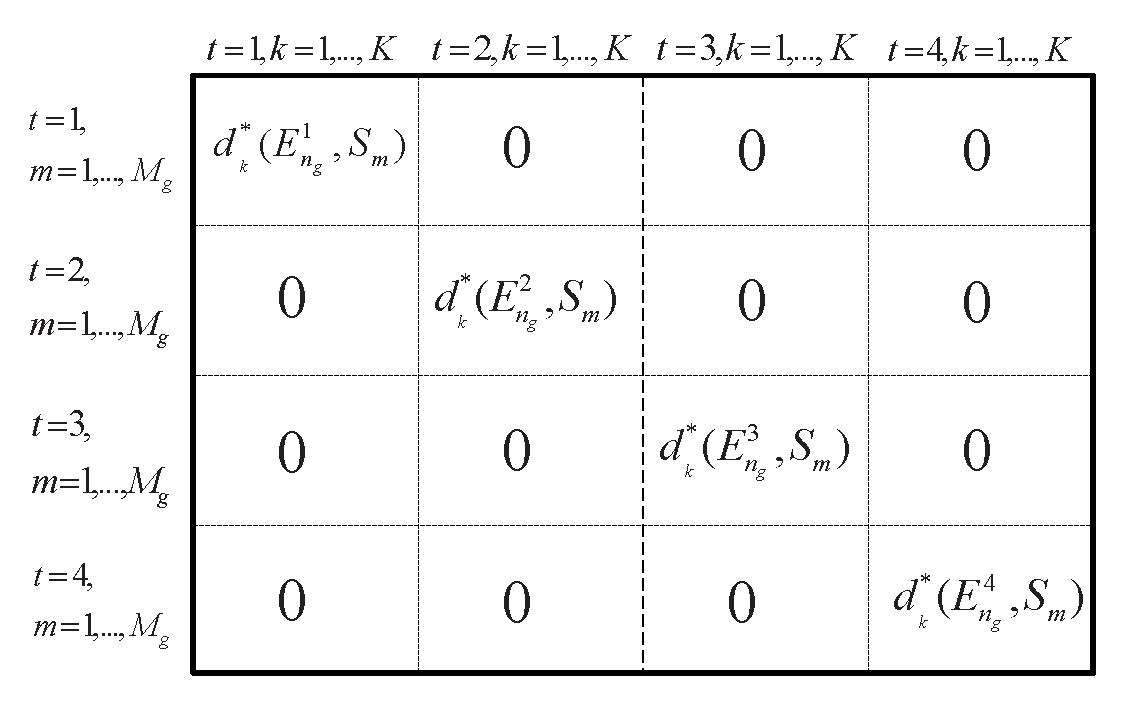
\includegraphics[scale=0.4]{2darray}\\
  \caption{A matrix representation of $d^*_{k}(E_{n_g}^t, S_{m_g})$.}\label{2darray}
\end{figure}

Let $\mathcal{A} =\{\{1\}, \{2\},..., \{4M_g\},$ $\{1, M_g+1, 2M_g+1, 3M_g+1\}, \{2, M_g+2, 2M_g+2, 3M_g+2\},...,\{M_g, 2M_g, 3M_g, 4M_g\}\}$ and $\mathcal{B} =\{\{1\}, \{2\},..., \{4K\}\}$. It is easy to verify that both $\mathcal{A}$ and $\mathcal{B}$ are good. According to Theorem \ref{IMD}, $d^*_{k}(E_{n_g}^t, S_{m_g})$ can be decomposed into $d^*_{k}(E_{n}^t, S_{m_g}), n\in n_g$ such that the four constraints in Theorem \ref{IMD} holds. In this case, the four constraints in Theorem \ref{IMD} can be restated as follows:
\begin{equation}\label{ImdConstraint1}
d^*_{k}(E_{n_g}^t, S_{m_g})=\sum_{n\in n_g} d^*_{k}(E_{n}^t, S_{m_g});
\end{equation}
\begin{equation}\label{ImdConstraint2}
\left\lfloor \frac{d^*_{k}(E_{n_g}^t, S_{m_g})}{|n_g|}\right\rfloor \leq d^*_{k}(E_{n}^t, S_{m_g}) \leq \left\lceil\frac{d^*_{k}(E_{n_g}^t, S_{m_g})}{|n_g|}\right\rceil;
\end{equation}
Constraint (3) in Theorem \ref{IMD} corresponds to two types of constraints as follows:
\begin{eqnarray}\label{ImdConstraint3}
\left\lfloor \frac{\sum_{k=1}^K d^*_{k}(E_{n_g}^t, S_{m_g})}{|n_g|}\right\rfloor &\leq& \sum_{k=1}^K d^*_{k}(E_{n}^t, S_{m_g})\\
&\leq&\left\lceil\frac{\sum_{k=1}^K d^*_{k}(E_{n_g}^t, S_{m_g})}{|n_g|}\right\rceil;\nonumber
\end{eqnarray}
\begin{eqnarray}\label{ImdConstraint4}
&&\hspace{-8mm}\left\lfloor \frac{\sum_{k=1}^K\sum_{t=1}^4 d^*_{k}(E_{n_g}^t, S_{m_g})}{|n_g|}\right\rfloor\hspace{1mm}\leq\hspace{1mm}\sum_{k=1}^K\sum_{t=1}^4 d^*_{k}(E_{n}^t, S_{m_g}) \\
&&\hspace{28mm}\leq\left\lceil\frac{\sum_{k=1}^K\sum_{t=1}^4 d^*_{k}(E_{n_g}^t, S_{m_g})}{|n_g|}\right\rceil;\nonumber
\end{eqnarray}
Constraint (4) in Theorem \ref{IMD} corresponds to just one type of constraints as follows:
\begin{eqnarray}\label{ImdConstraint5}
\left\lfloor \frac{\sum_{m_g=1}^{M_g} d^*_{k}(E_{n_g}^t, S_{m_g})}{|n_g|}\right\rfloor &\leq& \sum_{m_g=1}^{M_g} d^*_{k}(E_{n}^t, S_{m_g})\\
&\leq& \left\lceil\frac{\sum_{m_g=1}^{M_g} d^*_{k}(E_{n_g}^t, S_{m_g})}{|n_g|}\right\rceil.\nonumber
\end{eqnarray}

Recall that $d^*_k(E_{n_g}^t, S_{m_g})$ satisfies the constraints (\ref{blockaggregateblockdecisionvariables1})(\ref{blockaggregatesuperblockconnect1}) (\ref{blockaggregatesuperspineblockconstraint1})(\ref{blockaggregatemiddlespineblockconstraint1}). Combined with the constraints (\ref{ImdConstraint1})-(\ref{ImdConstraint5}), it is easy to verify that $d^*_{k}(E_n^t, S_{m_g}), n\in n_g$ satisfy the constraints
(\ref{blockaggregateblockdecisionvariables2})(\ref{blockaggregatesuperblockconnect2})(\ref{blockaggregatesuperspineblockconstraint2})(\ref{blockaggregatemiddlespineblockconstraint2}) in (\ref{individualserverblockdecomposition}).

After proving the feasibility of (\ref{individualserverblockdecomposition}), we can use either the ILP based approach or the min-cost-flow based approach developed in Section \ref{deaggregationalgorithmsection} to solve (\ref{individualserverblockdecomposition}). We do not elaborate it here any more.

\subsection{Spine Block Decomposition}
Now, we have accomplished patch-panel decomposition and server block decomposition, and proved that the decomposed variables $d^*_{k}(E_{n}^t, S_{m_g})$ satisfy the constraints (\ref{blockaggregateblockdecisionvariables2})-(\ref{blockaggregatemiddlespineblockconstraint2}). Once we accomplish spine block decomposition, we would obtain $d^*_{k}(E_{n}^t, S_{m})$ satisfying constraints (\ref{blockdecisionvariables})-(\ref{middlespineblockconstraint}). The details of spine block decomposition is very similar to server block decomposition, and thus we will not elaborate here.

\end{document}